\documentclass[12pt,a4paper]{report}

\usepackage{styles/dolgozat}

\usepackage{listings}
\usepackage{styles/python}

\usepackage{hyperref}

\begin{document}

\pagestyle{empty} %a címlapon ne legyen semmi=empty, azaz nincs fejléc és lábléc

% A Miskolci Egyetem címere
{\large
\begin{center}
\vglue 1truecm
\textbf{\huge\textsc{Szakdolgozat}}\\
\vglue 1truecm

\includegraphics[width=4.8truecm, height=4truecm]{images/me_logo.png}\\
\textbf{\textsc{Miskolci Egyetem}}
\end{center}}

\vglue 1.5truecm %függõleges helykihagyás

% A szakdolgozat címe, akár több sorban is
{\LARGE
\begin{center}
\textbf{Kiterjesztett valóság alapú prezentációs szoftver készítése}
\end{center}}

\vspace*{2.5truecm}
% A hallgató neve, évfolyam, szak(ok), a konzulens(ek) neve
{\large
\begin{center}
\begin{tabular}{c}
\textbf{Készítette:}\\
Nagy Dániel Zoltán\\
Programtervező informatikus
\end{tabular}
\end{center}
\begin{center}
\begin{tabular}{c}
\textbf{Témavezető:}\\
Piller Imre
\end{tabular}
\end{center}}
\vfill
% Keltezés: Hely, év
{\large
\begin{center}
\textbf{\textsc{Miskolc, 2020}}
\end{center}}

\newpage


\newpage

\pagestyle{empty}

%Feladatkiiras
\begin{flushleft}
\textsc{\bfseries Miskolci Egyetem}\\
Gépészmérnöki és Informatikai Kar\\
Alkalmazott Matematikai Intézeti Tanszék\hspace*{4cm}\hfil \textbf{Szám:}
\end{flushleft}
\vskip 0.5cm
\begin{center}
\large\textsc{\bfseries Szakdolgozat Feladat}
\end{center}
\vskip 0.5cm
Szakdolgozó Neve (N3P7UN) programtervező informatikus jelölt részére.\newline

\noindent\textbf{A szakdolgozat tárgyköre:} kulcsszavak, hasonlók\newline

\noindent\textbf{A szakdolgozat címe:} A dolgozat címe\newline

\noindent\textbf{A feladat részletezése:}

\medskip

\emph{Ide kell a feladatkiírásban szereplő szöveget betenni.}

\medskip

\emph{(Kisebb tagolás lehet benne, hogy jól nézzen ki.)}

\vfill

\noindent\textbf{Témavezető:} Piller Imre (egyetemi tanársegéd) \newline

% \noindent\textbf{Konzulens(ek):} (akkor kötelezõ, ha a témavezetõ nem valamelyik matematikai tanszékrõl való; de persze lehet egyébként is)\newline

\noindent\textbf{A feladat kiadásának ideje:}\newline

%\noindent\textbf{A feladat beadásának határideje:}

\vskip 2cm

\hbox to \hsize{\hfil{\hbox to 6cm {\dotfill}\hbox to 1cm{}}}

\hbox to \hsize{\hfil\hbox to 3cm {szakfelelős}\hbox to 2cm{}}

\newpage

\vspace*{1cm}  
\begin{center}
\large\textsc{\bfseries Eredetiségi Nyilatkozat}
\end{center}
\vspace*{2cm}  

Alulírott \textbf{Szakdolgozó Neve}; Neptun-kód: \texttt{N3P7UN} a Miskolci Egyetem Gépészmérnöki és Informatikai Karának végzős Programtervező informatikus szakos hallgatója ezennel büntetőjogi és fegyelmi felelősségem tudatában nyilatkozom és aláírásommal igazolom, hogy \textit{Szakdolgozat Címe}
című szakdolgozatom saját, önálló munkám; az abban hivatkozott szakirodalom
felhasználása a forráskezelés szabályai szerint történt.\\

Tudomásul veszem, hogy szakdolgozat esetén plágiumnak számít:
\begin{itemize}
\item szószerinti idézet közlése idézőjel és hivatkozás megjelölése nélkül;
\item tartalmi idézet hivatkozás megjelölése nélkül;
\item más publikált gondolatainak saját gondolatként való feltüntetése.
\end{itemize}

Alulírott kijelentem, hogy a plágium fogalmát megismertem, és tudomásul veszem, hogy
plágium esetén szakdolgozatom visszautasításra kerül.

\vspace*{3cm}

\noindent Miskolc, \hbox to 2cm{\dotfill} .év \hbox to 2cm{\dotfill} .hó \hbox to 2cm{\dotfill} .nap

\vspace*{3cm}

\hspace*{8cm}\begin{tabular}{c}
\hbox to 6cm{\dotfill}\\
Hallgató
\end{tabular}



\newpage

\noindent 1.

\begin{tabular}{cl}
&szükséges (módosítás külön lapon) \\
A szakdolgozat feladat módosítása& \\
& nem szükséges\\
&\\
\hbox to 4cm{\dotfill}&\multicolumn{1}{c}{\hbox to 5cm{\dotfill}}\\
dátum& \multicolumn{1}{c}{témavezető(k)}
\end{tabular}
\vskip1.5mm

\noindent 2. A feladat kidolgozását ellenőriztem:

\vskip1.5mm

\begin{tabular}{l@{\hspace*{4cm}}l}
témavezető (dátum, aláírás):& konzulens (dátum, aláírás):\\
\dotfill&\dotfill\\
\dotfill&\dotfill\\
\dotfill&\dotfill
\end{tabular}

\vskip1.5mm

\noindent 3. A szakdolgozat beadható:

\vskip1.5mm

\begin{tabular}{@{\hspace*{1.3cm}}c@{\hspace*{2.1cm}}c}
\hbox to 4cm{\dotfill}&\multicolumn{1}{c}{\hbox to 5cm{\dotfill}}\\
dátum& \multicolumn{1}{c}{témavezető(k)}
\end{tabular}

\vskip1.5mm

\noindent 4.
\begin{tabular}[t]{@{}l@{\hspace*{1mm}}l@{\hspace*{1mm}}l@{}}
A szakdolgozat& \hbox to 3.5cm{\dotfill} &szövegoldalt\\
              & \hbox to 3.5cm{\dotfill} &program protokollt (listát, felhasználói leírást)\\
              &\hbox to 3.5cm{\dotfill}   &elektronikus adathordozót (részletezve)\\
              &\hbox to 3.5cm{\dotfill} & \\
              &\hbox to 3.5cm{\dotfill} &egyéb mellékletet (részletezve)\\
              &\hbox to 3.5cm{\dotfill} &\\
\end{tabular}
\newline tartalmaz.

\vskip1.5mm

\begin{tabular}{@{\hspace*{1.3cm}}c@{\hspace*{2.1cm}}c}
\hbox to 4cm{\dotfill}&\multicolumn{1}{c}{\hbox to 5cm{\dotfill}}\\
dátum& \multicolumn{1}{c}{témavezető(k)}
\end{tabular}

\noindent 5.

\begin{tabular}{ll}
&bocsátható\\
A szakdolgozat bírálatra& \\
& nem bocsátható\\
\end{tabular}

\vskip1.5mm

\noindent A bíráló neve: \hbox to 8cm{\dotfill}

\vskip4mm

\begin{tabular}{@{\hspace*{1.3cm}}c@{\hspace*{2.1cm}}c}
\hbox to 4cm{\dotfill}&\multicolumn{1}{c}{\hbox to 5cm{\dotfill}}\\
dátum& \multicolumn{1}{c}{szakfelelős}
\end{tabular}

\noindent 6.
\begin{tabular}[t]{@{}l@{\hspace*{1mm}}l@{\hspace*{1mm}}l@{}}
A szakdolgozat osztályzata& &\\
&a témavezető javaslata:& \hbox to 3cm{\dotfill}\\
&a bíráló javaslata:& \hbox to 3cm{\dotfill}\\
&a szakdolgozat végleges eredménye:& \hbox to 3cm{\dotfill}
\end{tabular}

\vspace*{4mm}

\noindent Miskolc, \hbox to 4.5cm{\dotfill} \hspace*{2.5cm}
\begin{tabular}[t]{cc}
\hbox to 6cm{\dotfill}\\
a Záróvizsga Bizottság Elnöke
\end{tabular}


\cleardoublepage
\pagenumbering{gobble}
\tableofcontents
\cleardoublepage
\pagenumbering{arabic}

\newpage

\pagestyle{fancy}

\Chapter{Bevezetés}

% TODO: Leírni, hogy ez miben lesz újabb, jobb mint az eddigiek?

% A fejezet célja, hogy a feladatkiírásnál kicsit részletesebben bemutassa, hogy miről fog szólni a dolgozat.
% Érdemes azt részletezni benne, hogy milyen aktuális, érdekes és nehéz probléma megoldására vállalkozik a dolgozat.

% Ez egy egy-két oldalas leírás.
% Nem kellenek bele külön szakaszok (section-ök).
% Az irodalmi háttérbe, a probléma részleteibe csak a következő fejezetben kell belemenni.
% Itt az olvasó kedvét kell meghozni a dolgozat többi részéhez.

% Ezek még csak ötletek/egy gyors vázlat

A kiterjesztett valóság adta lehetőségek feltérképezése egy izgalmas kutatási terület. Szorosan összefonódik a képfeldolgozás, az ember-gép interakció (HCI) témakörökkel és ezáltal a gépi tanulásos témakörrel is. Vagyis kutatási területek széles skáláját érinti, amelyekkel manapság kiemelkedően sok cikk foglalkozik. Egy rendkívül izgalmas témakör, rengeteg lehetőséggel.

A dolgozatom feladataként egy olyan megoldás után kutatok a fent említett témakörökön belül, mely segítségével össze lehetne állítani egy elsősorban prezentációs szoftverként használatos alkalmazást, kihasználva a témakörökben rejlő lehetőségeket, a technikai korlátainkat figyelembe véve. A programom használatával a prezentáló személy a videófolyamra illesztett virtuállis elemek segítségével mutathatja be a témakört, a gesztusai segítségével vezérelheti a prezentáció menetét. A programom, felhasználási területét tekintve elsősorban élő közvetítések, konferenciahívások alkalmával lehetne hasznos. Így tehát a hagyományos értelemben vett prezentációs formákat nem célszerű helyettesíteni vele. Viszont az online felületen történő alkalamazása számos előnnyel járhat. Segítségével látványos, újszer előadásokat lehetne tartani.

A koncepciót igyekeztem a technikai lehetőségekhez mérten összeállítani. A későbbiekben megemlített korábbi kutatásokból láthatjuk, hogy előszeretettel használnak különféle segédeszközöket, mint például a mélységérzékelővel is ellátott \textit{Kinect} kamerarendszert. Az ilyen megoldások hátránya egyértelműen az eszközfüggőség, hiszen ezen szoftverek használatához elengedhetetlen ezen eszközök megléte. Az ilyen eszközökből eredő hibákkal is kénytelenek vagyunk együtt élni, mint például a \textit{Kinect}-re jellemző alacsony felbontás. Az elkészített programomhoz csupán egy kameraeszközre van szükségünk, ami akár lehet egy laptop egyszerű webkamerája is.

A dolgozat elején rövid ismertetők formájában bemutatásra kerülnek a témához kapcsolódó fogalmak, mint a kiterjesztett valóság, a prezentációs szoftverek, a képfeldolgozás és a gépi tanulás. Majd a definiált gesztusokról és lehetséges megvalósítási módjairól, a program működési módjáról olvashatunk áttekintő leírást. Ezt követi a programomban található virtuális elemek (widgetek) megvalósítási módjainak részletezése.

A megvalósítás fejezetben az elkészített implementációról olvashatunk pontos leírást, bemutatva az \texttt{arpt} csomag felépítését és a program szerkezetét.

A dolgozatot végül két darab példa prezentációval kívánom zárni, melyeken keresztül bemutatom az elkészített programom lehetséges felhasználási módját, működését.

\Chapter{Koncepció}

\Section{Kiterjesztett valóság}

% TODO: A dolgozat témája hogyan kapcsolódik hozzá, és hogy általában mit értünk alatta.

\Section{Prezentációs szoftverek}

% TODO: Megnézni 3-6 hasonló szoftvert. Készülhet hozzá összehasonlító táblázat, képernyőképek.

\Section{Valós idejű videó annotálás}

% TODO: OpenCV-ről néhány dolgot megemlíteni.

Az \textit{OpenCV} egy \textit{open source}, elsősorban valós idejű számítógépes látás megvalósítására támogatást nyújtó, magas tudású függvénykönyvtár. Számos képfeldolgozó algoritmus található benne, melyek implementációjánál a fejlesztők a lehető legjobb teljesítmény elérésére törekedtek.

Az \textit{OpenCV} eredetileg C és C++ nyelven íródott, de különböző nyelveket is támogat, mint például a \textit{Python}-t, \textit{Ruby}-t, \textit{Matlab}-ot, stb\ldots
Platformfüggetlen, így \textit{Linux}-on, \textit{Windows}-on és \textit{Mac OS X} rendszereken is használható. Lehetőséget nyújt továbbá a párhuzamosításra is a \textit{CUDA} és az \textit{OpenCL} technológiák segítségével és tartalmaz egy általános célú gépi tanulásos könyvtárat is, melyek tovább szélesítik a felhasználási területeinek körét. \cite{bradski2008learning}

Videófolyamok feldolgozásához is hasonló eljárásokat alkalmazhatunk, mint az önálló képek esetében. A videó képkockáit iteratív módon dolgozhatjuk fel, képkockáról képkockára. A videó két forrásból származhat: fájból és külső eszközből (pl.: webkamera képe). Az \textit{OpenCV}-ben mindkét esetben először definiálnunk kell egy olvasó eszközt. Ezt \textit{Python} esetében a \texttt{cv2.VideoCapture()} metódussal érhetjük el. Fájlból történő olvasás esetén paraméterként a fájl elérési útvonalára kell hivatkozni, külső eszköz esetén pedig az eszköz \textit{index}-ével történik a hivatkozás. Ha egyetlen ilyen eszköz áll rendelkezésünkre, akkor a 0-ás indexet is használhatjuk, hiszen az az első elérhető eszközre mutató index.
Az eszköz definiálása után a \texttt{.read()} metódusával olvashatjuk ki a képkockákat. A metódus meghívásakor visszatérési értékként megkapjuk a soron következő képkockát és egy értéket, amely az olvasás sikerességéről tájékoztat bennünket. A metódus meghívásakor a videóolvasó pointerét is inkrementáljuk, így a következő \texttt{.read()} meghívásakor már a soron következő képkockát olvashatjuk ki a videófolyamból. Ha már nem kívánjuk tovább használni az adott erőforrást, akkor a \texttt{.release()} metódusával szabadíthatjuk fel azt.

\Section{Gépi tanulás}

SciKit Learning

\Chapter{Gesztusok}

\Section{Felismerendő gesztusok}

A szoftver használata közben a prezentáló személy különféle gesztusok segítségével irányíthatja a prezentáció menetét és szintén gesztusok segítségével léphet kapcsolatba a videófolyamon megjelenő virtuális elemekkel. A felhasználó a karjai segítségével valósíthatja meg a mozdulatokat. A gesztusokat az alábbi kategóriákba sorolhatjuk:

\begin{itemize}
	\item \textbf{Sweep}: Egyenes vonalú mozgás, pl.: kézfej végighúzása a képtartományon. A mozgásnak van iránya és két képkocka között megfigyelhető a hossza is.
	\item \textbf{Shift}: Bizonyos virtuális elemek közvetlenül is reagálnak a környezetükben történő mozgásra. Az ilyen elemek az irányukba történő mozgással megegyező irányú mozgással reagálnak. Vagyis a prezentáló személy például a kezei segítségével egyszerűen eltolhatja az adott virtuális elemet. Az ilyen elemeket vezérlő gesztusokat \textit{Shift}-nek nevezhetjük el.
	\item \textbf{Blink}: Az ujjak gyors ökölbe zárása vagy a tenyér széttárásának mozdulata.
	\item \textbf{Drag and Drop}: Bizonyos virtuális elemeket a prezentáló személy képes megfogni, majd odébbhúzni és elengedni. A funkció eléréséhez a prezentálónak az ún. \textit{Drag and Drop} mozgássorozatot kell végrehajtania. Két \textit{Blink} gesztus között szabadon mozgathatja az "elkapott" elemet, majd végül a kívánt helyére teheti azt.
	\item \textbf{Rotation}: A videófolyamon történő örvénylő mozgás, ami akár több ponton is megfigyelhető. Ez lehet például karlendítés, körvonal/ív menti mozgás, tenyerek forgatása.
	\item \textbf{Többpontos kezelés}: A képen lévő összefüggő, nagyobb elmozdulások keresése, \textit{Blob}-ok alapján. Több pont egymáshoz képesti vizsgálata különféle szempontok alapján.
	\item \textbf{Symbol}: Levegőbe leírt szimbólumok, melyek segítségével további funkciókat érhet el a felhasználó.
\end{itemize}

\Section{Képek és vektor mezők}

% A feldolgozás folyamata ábra
% Videófolyam -> két kép kiragadása -> Elmozdulásértékek számítása

A videófolyamon megfigyelhető mozgást a további számítások elvégzéséhez először érzékelnünk kell. Az elmozdulások becslésére az ún. \textit{MotionFlow}/\textit{Optical Flow} technikák tűnnek a legalkalmasabbnak. Egy kiemelkedő és széles körben elterjedt eljárás a Bruce D. Lucas és Takeo Kanade által kidolgozott módszer, melynek implementálása az \textit{OpenCV}-ben is megtalálható.

A Lucas-Kanade módszer dedikált pontok követésére hivatott. Ha a videófomlyaból kiemelünk két képkockát, melyek között az eltelt idő kicsi, a módszer képes megbecsülni a két képkockán elhelyezkedő kijelölt pontok pozíciójának a változását, vagyis megadja a pontok elmozdulás vektorait. A módszer azon a megállapításon alapszik, hogy a videófolyamon egy kijelölt pont és a körülötte lévő pixelek halmaza közel azonos intenzitású $(I)$ a vizsgált időintervallumban. Ha a ponthoz tartozó valós objektum elmozdul a korábbi helyzetéről és az általa képviselt új pont a vizsgálandó terület tartományába esik, akkor a módszer képes becslést adni a vizsgált pont új helyzetére a videófolyamon. A módszer használatánál feltételezzük azt is, hogy a videófolyamon megfigyelhető mozgás viszonylag lassú, vagyis két képkockát vizsgálva az új pont nem eshet kívül a vizsgált pont tartományából. A módszer tetszőleges pontok halmazára alkalmazható. Elsősorban szürkeárnyalatos képekre használatos, de a megfelelő paraméterek megválasztása mellett színes képekre is használható. Színinformációk használata mellett pontosabb eredményt kaphatunk, hiszen ilyenkor egy-egy pont több információt hordozna, viszont a számításigény várhatóan erősen megnövekedne. 

Vegyünk egy pixelt az összehasonlítandó két képkocka egyikéből és jelöljük $I(x,y,t)$-vel, ahol $x,y \in \mathbb{R}$ a pixel pozíciója, $t$ pedig az idő. Tegyük fel, hogy a vizsgálandó pixel $(dx, dy)$ távolsággal elmozdul a következő képkockán megfigyelve $dt$ idővel később. Mivel ezek a pixelek ugyanannak a valós objektumnak a vetületei, ezért feltételezzük, hogy az intenzitásértékük nem változott. Így
\begin{align*}
I(x,y,t) = I(x+dx,y+dy,t+dt)
\end{align*}
Ezután vegyük a jobb oldali kifejezés Taylor-sor közelítését, távolítsuk el a közös kifejezéseket, majd osszunk $dt$-vel. Így a következő egyenletet kapjuk:
\begin{align*}
f_xu+f_yv+f_t=0
\end{align*}
ahol:
\begin{align*}
f_x = \frac{\partial f}{\partial x} &; f_y = \frac{\partial f}{\partial y}\\
u = \frac{dx}{dt} &; v = \frac{dy}{dt}
\end{align*}
A fenti egyenlet \textit{Optical Flow egyenletnek} hívjuk, melyben $f_x$ és $f_y$ kép gradiensek. Hasonlóan, $f_t$ az idő gradiense. De $(u,v)$, vagyis az elmozdulás vektorok ismeretlenek. Ezen kétismeretlenes egyenlet megoldására számos módszer létezik, ezek egyike a \textit{Lucas-Kanade} módszer.

Korábban említettük, hogy a vizsgálandó pont és az őt körülvevő pontok halmazai közel azonos intenzitásértékekkel rendelkeznek a megfigyelés időtartamában. Vegyünk például egy $3 \times 3$-as foltot a vizsgálandó pixel körül. A megállapítás alapján feltételezhetjük, hogy ezen tartományba eső pixelek elmozdulása hasonló lesz. Megkereshetjük az $(f_x,f_y,f_t)$-ket ezekre a pontokra. Így 9 darab kétismeretlenes egyenletet kapunk, amely túlhatározott.

Egy jobb megoldás kapható a \textit{Legkisebb négyzetek módszerének} segítségével. A végső megoldást a következő egyenlettel szemléltethetjük, amely egy két egyeletes-kétismeretlenes probléma:
\begin{align*}
\bmatrix u \\ v \endbmatrix = {\bmatrix \sum_{i}(f_{x_i})^2 & \sum_{i}f_{x_i}f_{y_i}\\ \sum_{i}f_{x_i}f_{y_i} & \sum_{i}(f_{y_i})^2 \endbmatrix}^{-1} \cdot \bmatrix -\sum_{i}f_{x_i}f_{t_i} \\ -\sum_{i}f_{y_i}f_{t_i} \endbmatrix
\end{align*}
Az \textit{OpenCV}-ben található implementáció ún. \textit{Gauss képpiramis}-ok használatával próbálja kiküszöbölni a nagy mozdulatok esetén fellépő hibás eredményeket, vagyis a vizsgálandó képeknek különböző felbontású változatait vizsgálja iteratívan a kisebb felbontástól az eredeti felbontásig haladva. A piramis mélysége tetszőleges, a legkisebb szint egyetlen pixelből is állhat. Kis felbontások mellett a nagyobb mozdulatok könnyebben azonosíthatóak, a piramis szélesebb szintjeihez közelítve, nagyobb felbontások mellett pedig a becslés pontosítása történik. \cite{lucas1981iterative} \cite{bradski2008learning}

\begin{figure}[h]
\centering
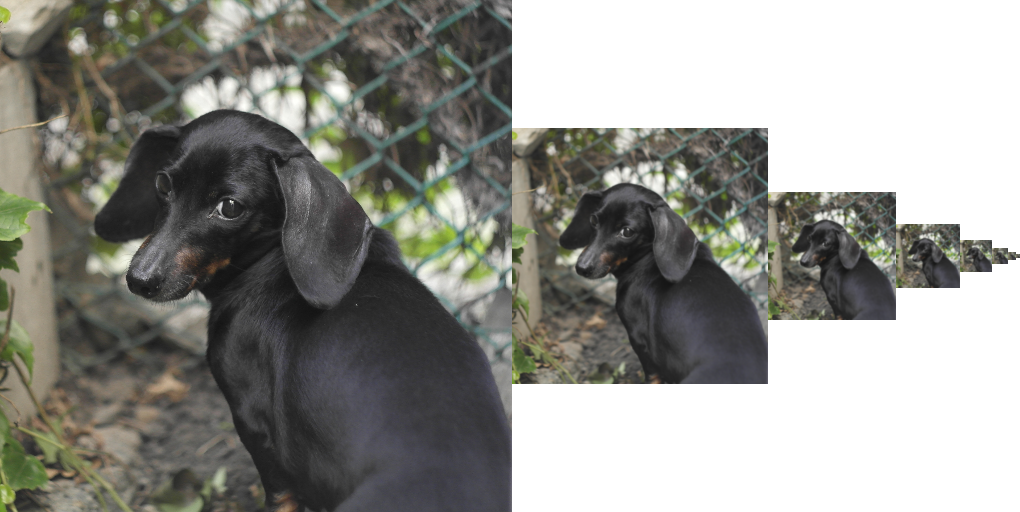
\includegraphics[width=7.65truecm, height=3.84truecm]{images/gauss_pyramid.png}
\caption{Gauss piramis}
\label{fig:gausspyramid}
\end{figure}

A módszer \textit{Spare Optical Flow}-t valósít meg, vagyis egymástól különálló pontokat vizsgál, ellentétben a \textit{Dense Optical Flow} módszerekkel, melyek a teljes kép vizsgálatával számolják ki az elmozdulás vektorokat. \cite{bradski2008learning} Az utóbbi módszerek számításigénye kifejezetten magas. Valós idejű alkalmazás esetén problémákba ütközhetünk gyengébb hardverek esetében. A mozgás valós idejű detektálására a \textit{Spare Optical Flow} módszerek is kielégítő eredményekkel szolgálnak, néhány trükk alkalmazása mellett. Ilyenek például a már említett \textit{kép-piramisok} használata a gyors mozgások pontos követésére és a vizsgálandó pontok kijelölésének a stratégiája is. A pontok kijelöléséhez egy rácsszerkezet használatát gondoltam a legmegfelelőbbnek, ahol a pontok a rács középpontjaiban helyezkednek el. A képtartományt ily módon egyenletesen fedik le a pontok, a további számításokat pedig ehhez tudjuk igazítani.

\Section{Rácspontok kezelése}

Az \textit{Optical Flow} eljárást tetszőleges számú pontra elvégezhetjük. Ha létrehozunk egy rácsszerkezetet fix pontokkal, akkor a képtartományt egyenletesen lefedhetjük a pontok halmazával.
Ezen pontokat felhasználva minden iterációban az éppen aktuális és az egyel korábbi szürkeárnyalatos képkockákra elvégezhetjük az eljárást és így minden esetben kapunk egy új ponthalmazt, amely az eljárás eredménypontjait tartalmazza. Az eredeti és az új pontok párjaiból egy vektormezőt kapunk.

\begin{figure}[h]
\centering
\frame{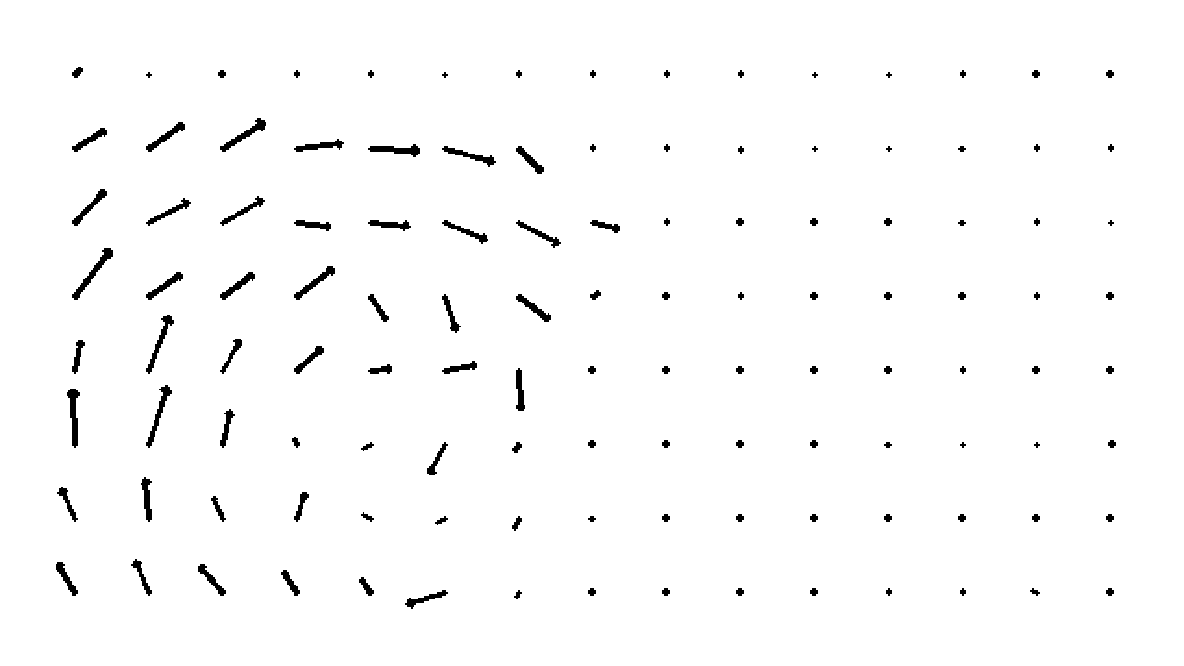
\includegraphics[width=11.2truecm, height=6.3truecm]{images/vectorField_screenshot.png}}
\caption{Képernyőfotó a vektormezőről, egy $8 \times 15$-ös rácsfelbontás mellett}
\label{fig:vectorfield}
\end{figure}

A kapott pontok párjaiból kiszámolhatjuk az elmozdulásvektorokat.

A mozgás detektálása rácspontok segítségével kevesebb számítást igényel, mintha minden pixel elmozdulását vizsgálnánk és az elmozdulás becslésére is elfogadható eredményeket kapunk.
A rács felbontását tetszőlegesen megadhatjuk. Minél nagyobb a felbontás, annál több pontot vizsgál a szoftver, ami nagyobb pontosságot is eredményez. Viszont a rácsfelbontás használata a futási időt is befolyásolja. Egy gyengébb hardver esetén nem ajánlott magas rácsfelbontás mellett futatnunk a programot, mivel tapasztalataim szerint jelentős lassulásra számíthatunk.

A rácspontok helyzetének meghatározásához elsősorban definiálnunk kell a rács felbontását és ismernünk kell a videófolyam felbontását is. Érdemes a képarány függvényében megválasztani a rács felbontásásnak értékeit. Pédául egy 16:9-es képarányú videófolyam esetén egy $9 \times 16$-es rács használata teljesen megfelelőnek tűnik, vagyis 9 sorban és 16 oszlopban lesznek elhelyezve a pontok az említett felbontás használata mellett. Ez 144 vizsgálandó pontot jelent.
A képtartomány széleit nem szükséges vizsgálnunk, hiszen a képből kilépő objektumok további helyzetét már nem tudjuk meghatározni és feltételezzük, hogy a lényeges mozgások nem a széleken történnek. Így érdemes egy bizonyos kereten belül elhelyeznünk a pontokat.

\bigskip

\noindent A következő algoritmus segítségével határozhatjuk meg a pontok helyzetét:

\medskip

\noindent \textbf{Rácspontok$\_$generálása}(@kép, @rács\_felbontás, @rács)\\
szélesség $\leftarrow$ kép.szélesség()\\
magasság $\leftarrow$  kép.magasság()\\
cella\_magasság $\leftarrow$ $\frac{\text{magasság}}{\text{rács\_felbontás}_0}$\\
cella\_szélesség $\leftarrow$ $\frac{\text{szélesség}}{\text{rács\_felbontás}_1}$\\
k $\leftarrow$ 0\\
\textbf{FOR} i $\leftarrow$ 0 \textbf{TO} $\text{rács\_felbontás}_0-1$ \textbf{DO}\\
\indent \textbf{FOR} j $\leftarrow$ 0 \textbf{TO} $\text{rács\_felbontás}_1-1$ \textbf{DO}\\
\indent \indent $\text{rács}_{k,0}$ $\leftarrow$ j $\times$ cella\_szélesség $+ \frac{\text{cella\_szélesség}}{2}$\\
\indent \indent $\text{rács}_{k,1}$ $\leftarrow$ i $\times$ cella\_magasság $+ \frac{\text{cella\_magasság}}{2}$\\
\indent \indent k $\leftarrow$ k + 1\\
\textbf{RETURN} rács

\Section{Hőtérkép}

A vektormező egyes pontjait vizsgálva szerkeszthetünk egy ún. \textit{Hőtérkép}-et, amelyben különböző intenzitásértékekkel jelöljük az egyes vektorok hosszait. Az általam definiált \textit{Hőtérkép} egy $n \times m$-es mátrix, ahol $n$ a vektormező sorainak, $m$ pedig az oszlopainak a száma. A \textit{Hőtérkép} minden eleme egy BGR (blue, green, red) hármas értékkel van ellátva. Ezen értékek jelölik az egyes elemek színét. A BGR színkódolás használata, a szokványos RGB helyett az \textit{OpenCV} egyik jellegzetessége.\\
Az értékek a következőképpen kerülnek kiszámításra:\\
\newline
\noindent \textbf{Hőtérkép$\_$kiszámítása}(@vektormező, érzékenység, @hőtérkép)\\ 
Input paraméter: vektormező (n$\times$m-es mátrix), érzékenység\\
Output paraméter: hőtérkép\\
\textbf{FOR} i $\leftarrow$ 1 \textbf{TO} Hossz(vektormező$_n$) \textbf{DO}\\
\indent \textbf{FOR} j $\leftarrow$ 1 \textbf{TO} Hossz(vektormező$_m$) \textbf{DO}\\
\indent \indent hőérték$_{ij}$ $\leftarrow$ hossz(vektormező$_{ij}$)*érzékenység\\
\indent \indent \textbf{IF} hőérték$_{ij}$ > 255\\
\indent \indent \indent \textbf{THEN} hőérték$_{ij}$ $\leftarrow$ 255\\
\indent \indent hőtérkép$_{ij}$ $\leftarrow$ (255-hőérték$_{ij}$, 0, hőérték$_{ij}$)\\
\textbf{RETURN} hőtérkép\\
\newline
0 pixel hosszúság esetén az adott indexű elem (255, 0, 0) értéket kap, vagyis kék színnel jelöljük. Ha egy adott vektor számított hőértéke eléri a 255-öt, a hozzá tartozó \textit{hőtérkép-érték} (0, 0, 255) intenzitásértéket kap, vagyis tiszta piros színnel fog megjelenni.
A \textit{érzékenység} értékkel állíthatjuk be, hogy mely vektorhosszakat vegyen a program figyelembe. Az érték megadja, hogy milyen mértékű legyen a vektorok nagyítása, befolyásolva ezzel a számított \textit{hőértéket}.
\begin{figure}[h]
\centering
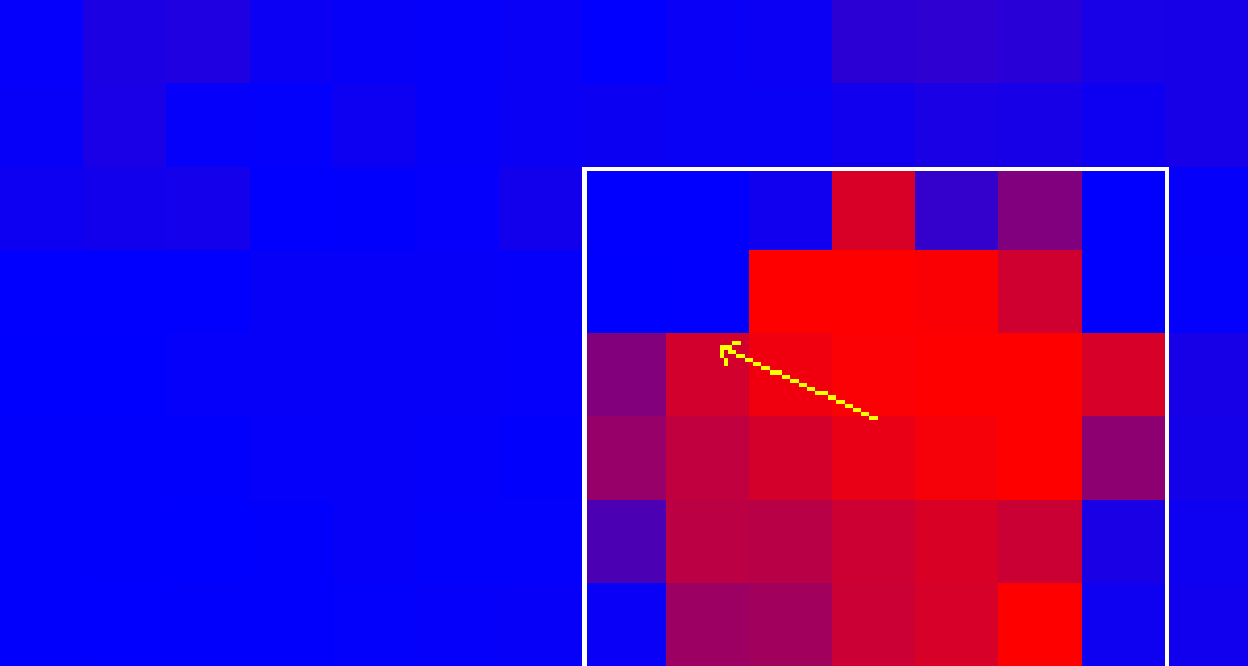
\includegraphics[width=11.2truecm, height=6.3truecm]{images/HeatMap_screenshot.png}
\caption{Képernyőfotó a hőtérképről}
\label{fig:heatmap}
\end{figure}
A három színcsatorna használata csupán megjelenítés szempontjából előnyös, mivel a kék és a piros szín elüt egymástól, így szabad szemmel nézve jobban meg tudjuk figyelni a kiszámított értékeket. Viszont a program számára a szürkeárnyalatos kép is elegendő információt hordoz, így a feldolgozás során a fent kikevert színértékeknek nincsen további jelentősége.

Az így kapott mátrixból ezután különféle információkat nyerhetünk ki. Az intenzitás értékeket vizsgálva meghatározhatjuk a nagyobb elmozdulások csoportjait. Ehhez küszöbölni kell a mátrixot, majd a kapott képen kontúrok keresésével meg lehet állapítani, hogy mely vektorok tartoznak egy csoportba. A csoportokat egy bizonyos intenzitás érték fölött érdemes keresni, vagyis az olyan vektorok összetartozó halmazai lehetnek érdekesek számunkra, amelyekben a vektorok hossza egy bizonyos határt elér. Az esetlegesen előforduló képzajok és az a videófolyamon megfigyelhető egyéb anomáliák miatt, amelyek a vektormező értékeire is hatással lehetnek, meg kell szabnunk a csoportok minimális területét. A megfelelően megválasztott értékek mellett a képzajból származó hibás értékek nem befolyásolják a program működését.
A \ref{fig:heatmap} ábrán megfigyelhető, hogy az összetartozó értékek fehér kerettel vannak jelölve. Továbbá a csoportok elmozdulásának irányai sárga nyilakkal vannak ábrázolva. A csoportokat külön-külön vizsgálva további értékes információkhoz juthatunk. Ilyen például az egyes csoportok iránya is, amelyet egy lokális eredővektor számításából kaphatunk meg. A csoportokat felhasználhatjuk további funkciók megvalósítására is, mint például a \textit{Többpontos kezelés}, a \textit{Rotation} és a \textit{Symbol}.

\Section{Gépi tanulásos módszerek, teljesítménymérések}

A dolgozatom programjához szükséges modellek betanításhoz felügyelt tanítási módszert kívánok alkalmazni, \textit{offline} adatkészletekkel. Az ilyen típusú tanító módszererek hátrányai közé sorolhatjuk a rugalmatlanságot is, vagyis az alkalmazóképesség hiányát is. Az \textit{online} tanulásos módszerek ezzel ellentétben sokkal jobban alkalmazkodnak, hiszen működés közben a valós világ éppen aktuális jellegzetességeihez igazítják magukat. Az \textit{online} módszerek előnye lehet a kisebb memória igény is, hiszen kevesebb adatmennyiség van jelen a futás során. Ez egyben a módszerek hátrányát is jelenti, mivel könnyen felejtenek az ilyen megoldások és a drasztikus, hirtelen változásokra rosszabbul reagálnak, mint az \textit{offline} módszerek. \cite{geron2019hands}

A tanítómintát két részre szokás bontani, tanító adatkészletre és teszt részre. A tanító adatkészletünk a modell tanítására szolgál, míg a teszt adatkészlet segítségével pedig a már betanított modellünk teljesítményét mérhetjük. A teszt adatkészlet elkülönítése azért szükséges, hogy betanítás után olyan adatokkal is tudjuk vizsgálni a modell teljesítményét, melyek nem egyeznek meg a tanítómintával. Így pontosabb eredményeket kaphatunk a teljesítményről, hiszen feltételezhetjük, hogy "élesben" is hasonlóan eredményeket fog szolgáltatni. Fontos a helyes arány megválasztása a felbontásnál, általánosan 70\% tanító és 30\% teszt adat javasolt. \cite{geron2019hands}

Az adatkészlet helyes mennyiségének meghatározása sok tényezőtől függhet, de belátható, hogy minél több adattal rendelkezünk az adott problémáról, annál kevésbé fognak érvényesülni az egyes osztályozó típusok előnyei. \cite{geron2019hands} Az adatok osztályok közti eloszlása is hatással lehet az osztályozó teljesítményére. Javasolt kiegyensúlyozott adatkészlettel dolgozni. Viszont az osztályozó hibáit bizonyos mértékig orvosolhatjuk az egyes osztályokon belül található adatok számának változtatásával. Az osztályozó teljesítményét tovább növelhetjük automatikus paraméterkereséssel, \textit{Grid-Search}-el is, amelyel az optimális paramétereket kívánjuk megtalálni. \cite{koesmarno2019class}

A program működése során felmerülő feladatokhoz a \textit{Random Forest} típusú osztályozót választottam, amely döntési fákat alkalmaz a részminták halmazán, majd átlagolás segítségével hozza meg a döntéseket. Az egyszerre több osztályozó segítségével történő osztályozást \textit{ensemble} \cite{geron2019hands}, vagyis együttes módszereknek nevezzük.

A betanított modell teljesítményének mérésére két módszert kívánok alkalmazni, a \textit{Cross-Validatiot} és a \textit{Confusion Matrix} ábrázolást.

\SubSection{Cross-Validation}

A \textit{$k$-hajtásos Cross-Validation} technika a mintát $k$ egyenlő részre osztja, majd egy ciklussal végigmegy a $k$-kon: a minta $k-1$ részével tanítja a modellt, majd a maradékon pedig ellenőrzi és kiértékeli az így beatanított modell teljesítményét. Így $k$ darab eredményt kapunk, melyet átlagából következtethetéseket vonhatunk le a modell teljesítményéről.

Például a \textit{Symbol}-hoz készített három osztállyal rendelkező 348 elemű adatkészletem 70\%-os (243 db) tanítómintájára, $k=5$ hajtással elvégzett \textit{Cross-Validation} teljesítménymérése a következő:
\begin{align*}
	k_1 &= 0.9388\\
	k_2 &= 0.9796\\
	k_3 &= 0.9592\\
	k_4 &= 0.9167\\
	k_5 &= 0.9792\\
	\bar{k} &= 0.9547
\end{align*}
Ahol $\bar{k}$ a minta átlaga.\\
Az eredményekhez érdemes hibát is számolni, majd segítségével konfidencia intervallumot megadni. Legyen például a konfidenciaintervallum 95\%-os és a hibát Standard hibaként tekintsük.
\begin{align*}
	\boldsymbol{CI}(95) = m (+/-) 1.96 \cdot \frac{s}{\sqrt[]{n}}
\end{align*}
Ahol $m$ a minta átlaga, $s$ a szórás, $n$ pedig a minta darabszáma.\\
Az eredmények alapján a betanított modellünk $95.47 (+/- 2.12)$\%-os pontossággal rendelkezik, vagyis ennyi valószínűséggel hoz helyes döntéseket. Hogy megvizsgáljuk, hogy mely esetekben téved a modellünk egy másik teljesítménymérő módszer segítségére lesz szükségünk, a \textit{Confusion Matrix} ábrázolásra.

\SubSection{Confusion Matrix}

\begin{figure}[h]
\centering
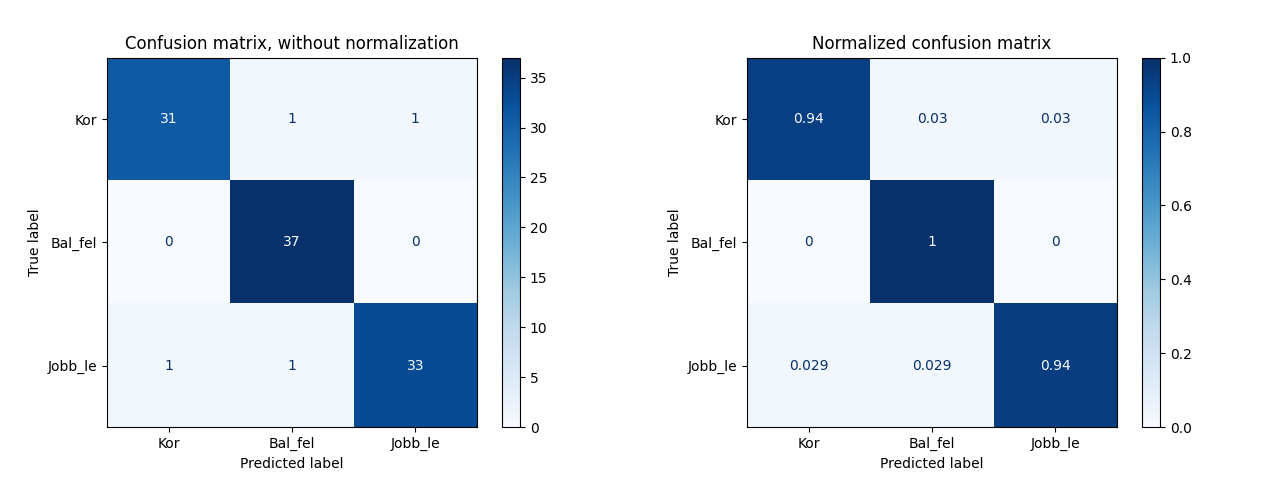
\includegraphics[width=\textwidth]{images/confusion_m.png}
\caption{\textit{Confusion Matrix}-ok a \textit{Symbol} adatkészletre}
\label{fig:confusionm}
\end{figure}

A teljesítménymérésnek egy másik módja lehet az úgynevezett \textit{Confusion Matrix} módszer. Segítségével meg lehet figyelni a helyes és hibás döntések eloszlását egy mátrix formájában.\cite{koesmarno2019class}
A már betanított modellünket a teszt adatkészlettel ellenőriztetjük, majd az eredmények alapján megszerkeszthetjük a mátrixunkat. Két fajta eredmény keletkezhet minden osztályban: Helyes becslés és hibás becslés. Mátrix soraiban az adatkészletben szerepő osztályok találhatók, míg oszlopaiban a becslések. Az általános \textit{Confusion Matrix} főátlójában a helyes becslések eloszlása figyelhető meg. Az átló alatti és feletti részeken pedig a hibás becslések, vagyis a hibás reosztályozások számai. A mátrixból jól leolvasható, hogy mely osztályokat kever össze az adott modell. A normalizált mátrix csupán arra szolgál, hogy nagy mennyiségű adatok mellett is jól kiolvashatóak legyenek az egyes osztályokra hozott becslések mértékei.
A \ref{fig:confusionm} ábrán megfigyelhető a \textit{Symbol} adatkészletre betanított modell, teszt mintahalmazzal való ellenőrzése \textit{Confusion Matrix} ábrázolással. Megfigyelhető, hogy milyen esetekben hozott hibás döntést a modellünk.

\Section{Kontrollpontok és vektorok számítása}

\SubSection{Sweep}

A \textit{Sweep} gesztus két tulajdonsággal írható le: A mozgás irányával és hosszával. A mozgás irányát egy $\vec{v}\in\mathbb{R^2}$ irányvektorral határozhatunk meg, amelyet a \textit{vektormező} globális eredővektoraként kapunk meg.
\begin{align*}
  \vec{v} = \sum_{i=1}^n\vec{u_i}
\end{align*}
, ahol $\vec{u}$ a teljes képre vett vektormező vektorai.\\
A mozgás hossza a vektormező vektorainak átlagos hosszában mérhető és pixelszámban fejezhető ki.
\begin{figure}[h]
\centering
\frame{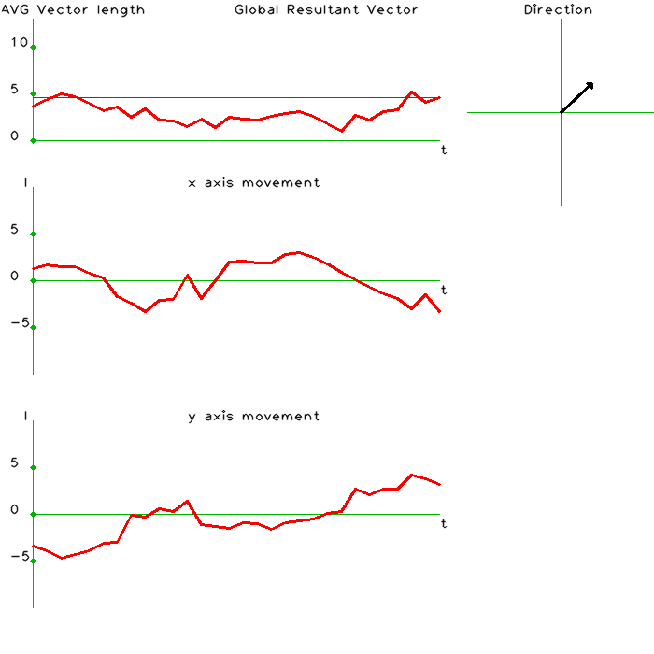
\includegraphics[width=8.0truecm]{images/ResultantPlot_screenshot.png}}
\caption{Képernyőfotó a globális eredővektor grafikonjáról}
\label{fig:resultantplot}
\end{figure}

Az ábrán megfigyelhető a globális eredő vektor hosszainak változása egy 30 képkockás \textit{csúszóablakban} és az éppen aktuális irányvektor is, valamint az $x$ és $y$ tengelyen megfigyelhető mozgások változásai is.

\SubSection{Shift}

A \textit{Shift} tulajdonsággal rendelkező virtuális elemeknek mindig van egy aktuális pozíciójuk $(x,y)$, szélességük és magasságuk $(w,h)$, illetve sebességértékük $v_{xy}$ (a két tengelyre vonatkozóan). A pozíciót a virtuális elem bal felső sarkának tekintsük.

A \textit{Shift} viselkedésének meghatározásához első lépésként az adott virtuális elem területére eső vektorokból $\vec{v}_l$  lokális irányvektort számolunk. Az elem területére eső vektorok meghatározható az elem pozíciója és a mérete alapján a következő módon:

Jelöljük $\boldsymbol P \in \mathbb{R}^2$-vel a virtuális elem pozícióját $(x,y)$, $\boldsymbol D \in \mathbb{R}^2$-vel pedig a dimenzióját (szélesség, magasság).
A rácspontok alapján kiszámolhatjuk a lépésközt is, ami rács első koordinátájának az összege lesz. Ezt jelöljük $\boldsymbol L \in \mathbb{R}$-el. 
\begin{align*}
	\boldsymbol L = \textit{rács}_{0,0} + \textit{rács}_{0,1}
\end{align*}
Ha rácsot háromdimenziós vektornak tekintjük, vagyis egy $n\times m$-es mátrixnak, ahol $n$ a rács sorait, $m$ pedig az oszlopait jelöli.\\
A részmátrix kezdőpozícióját jelöljük $\boldsymbol {RM}poz \in \mathbb{R}^2$-vel,\\
dimenzióját pedig $\boldsymbol {RM}dim \in \mathbb{R}^2$-vel.
\begin{align*}
	\boldsymbol {RM}poz &= \left\lfloor \frac{\boldsymbol P}{\boldsymbol L} \right\rfloor\\
	\boldsymbol {RM}dim &= \left\lfloor \frac{\boldsymbol D}{\boldsymbol L} \right\rfloor
\end{align*}
Jelöljük $\vec{u}$-val a vektormező irányvektorait.
\begin{align*}
  \vec{v_l} &= \frac{\sum_{i=\boldsymbol {RM}poz_1}^{\boldsymbol {RM}dim_1} \sum_{j=\boldsymbol {RM}poz_0}^{\boldsymbol {RM}dim_0} \vec{u}_{ij}}{\boldsymbol {RM}dim_0 \cdot \boldsymbol {RM}dim_1}
\end{align*}
Így megkaptuk a $\vec{v_l}$ lokális irányvektort, amely egyben az elem elmozdulásvektora is. Segítségével kiszámolhatjuk az elem sebességét:
\begin{align*}
  v_{xy} = v_{xy} + \frac{\vec{v}_l}{\boldsymbol {RM}dim_0 \cdot \boldsymbol {RM}dim_1} \cdot \textit{gyorsulás}
\end{align*}
, ahol $\textit{gyorsulás} > 0$.\\
Az elem pozíciója ($\boldsymbol P$) a sebesség függvényében változik.
\begin{align*}
  \boldsymbol P = \boldsymbol P+v_{xy}
\end{align*}
A sebesség értéket minden iteráció végén tompítani kell, hogy a kezelt virtuális elem meg tudjon állni egy bizonyos ponton. Ha az adott elemet nem éri tovább erő, akkor a tompítás lassulást eredményez, a sebesség csökkenni fog. Olyan hatást is el tudunk érni egy helyesen megválasztott értékkel, mintha az eltolás után az elem csúszós felületen mozogna és így fokozatosan lassul le az iterációk során.
\begin{align*}
  v_{xy} = v_{xy} \cdot \textit{tompítás}
\end{align*}
, ahol $0 \leq \textit{tompítás} < 1$

\SubSection{Blink}

A \textit{Blink} gesztusok felismerésére elsősorban egy ún. \textit{Frame differencing} technikát kell alkalmaznunk.
Ehhez a videófolyam aktuális képkockájának és az eggyel korábbi képkockájának abszolút különbségét kell meghatározni, majd az így kapott képen küszöbölést kell végrehajtani. Eredményképp egy olyan képet kapunk, amelyen az elmozdulás figyelhető meg fehér színnel jelölve. A keletkezett képen különféle alakzatok alakulhatnak ki. Az egyes mozdulatok hasonló nyomot hagynak maguk után. Így tehát egy \textit{Blink} mozdulat leadásakor jellegzetes mintázat rajzolódik ki.

\begin{figure}[h]
\centering

\includegraphics[width=4truecm, height=4truecm]{images/Grab_screenshot.png}
\caption{Egy Blink mozdulat pillanatképe}
\label{fig:blink}
\end{figure}

A \textit{Frame differencing} technika a teljes képtartományra vonatkozik, minden iterációban elvégezhetjük, hogy a videfolyamon történő mozgásról információkat kapjunk. A \ref{fig:blink} ábrán megfigyelhető, hogy nem csupán a legfrissebb két képkocka adatai vannak jelen a képen. Ezt a jelenséget egy keverési technikával érhetjük el. A korábbi mozdulatok rajzolatai alacsonyabb intenzitás értékekkel jelennek meg, míg a legfrissebb értékek 255 intenzitással vannak jelölve.

A gesztus detektálásához rögzített hosszúságú jellegvektorokra lesz szükségünk. A \textit{Frame differencing} technika képének dimenzió megegyeznek a videófolyam felbontásával. Így például $640\times480$ felbontás mellett 307200 hosszúságú jellegvektorokat kapunk. A gesztus ily módon történő detektálása nem a legoptimálisabb megoldás. A \textit{Frame differencing} kép felbontásának csökkentésével pedig romolhat az információ minősége is.

A \textit{Blink} gesztusról feltételezhetjük, hogy a videófolyam egy kis területén fog jelentkezni. A terület meghatározásához segítségül kell hívnunk a \textit{Hőtérkép} által meghatározott csoportokat. A gesztus kiadásának pillanatában feltételezhetjük, hogy a \textit{Blink}-en kívül más egyéb mozgás nem figyelhető meg a videófolyamon, amely a \textit{Hőtérkép} számításánal újabb csoportokat jelentene. Így tehát a \textit{Blink} további vizsgálatának előfeltétele, hogy a \textit{Hőtérképen} csupán egyetlen összefüggő csoport helyezkedjen el.
\begin{figure}[h]
\centering
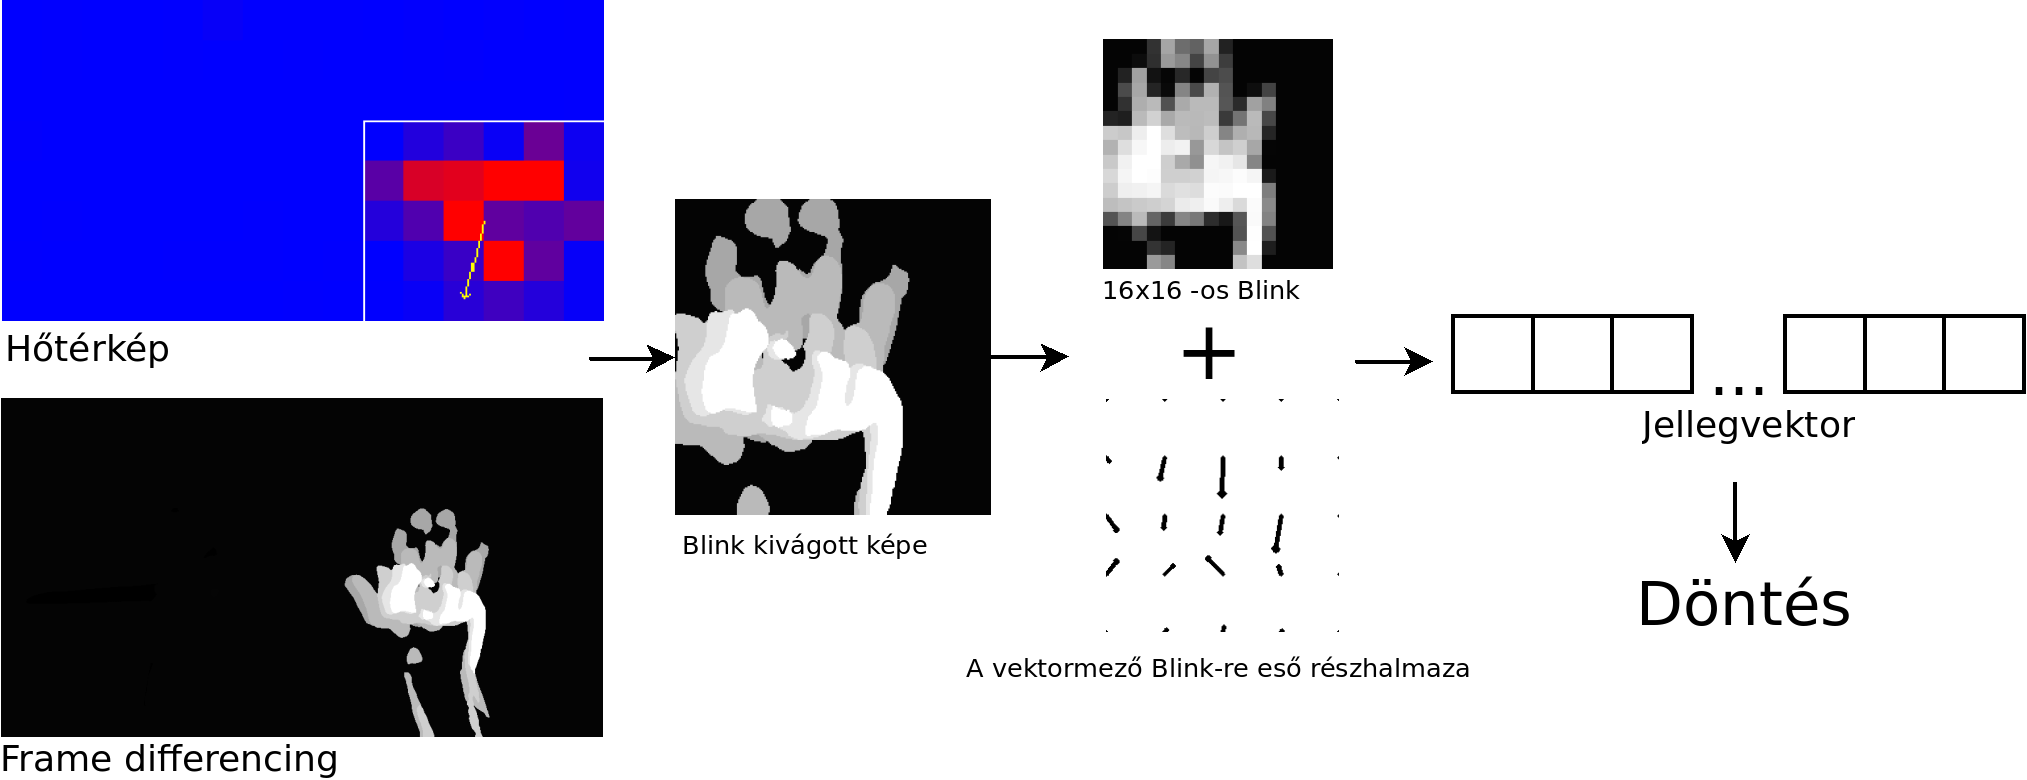
\includegraphics[width=\textwidth]{images/blink_flow.png}
\caption{A gesztus detektálásának folyamata}
\label{fig:blinkflow}
\end{figure}

A csoport változásait ezután figyelemmel kísérjük, a tulajdonságait egy szűrési feltétel után rögzítjük. Mivel a \textit{Blink} gesztus várhatóan a vektormező egy viszonylag kis területen figyelhető meg, ezért egy bizonyos \textit{Hőtérkép-csoport} méret fölött nem érdemes további vizsgálatokat végrehajtani. Ha a \textit{Hőtérképen} megfigyelhető csoport területe meghaladja a 25 pixelt, akkor arról a csoportról feltételezhetjük, hogy nem tartalmaz \textit{Blink} gesztust. Természetesen ez a mennyiség rácsfelbontásokként változhat. Egy nagy sűrűségű rácson valószínűleg már alacsony lenne ez az érték, viszont az ajánlott rácsfelbontás mellett jól működik. Mint korábban kifejtettem, nem érdemes túl sűrű rácsot alkalmazni, így a területre megszabott korlát az indokolt rácsfelbontásokig megfelelőnek tűnik.

Ha a területre vonatkozó szűrés eredményes lesz, meghatározhatjuk a \textit{Blink} gesztus középpontját. A szűrésen átesett csoport nem minden esetben négyzetes. A rögzített jellegvektor hossz szükségessége miatt minden esetben egy $5\times5$-ös részmátrixot kell meghatároznunk a \textit{Vektormezőre} nézven. A részmátrix középpontját a \textit{Hőtérképből} kinyert csoport középpontja adja. A mátrix szélein és a sarkoknál, az indexelés helyessége miatt meg kell szabnunk, hogy a középpont minimum 2 lépés távolságra lehet a szélektől. Ha esetleg ez nem teljesülne, a legközelebbi helyes pontot jelöljük ki a \textit{Blink} gesztus középpontjának. A részmátrix segítségével meghatározhatjuk a \textit{Vektormező} $5\times5$-ös csoportra eső irányvektorait is. A gesztus területére eső irányvektorokat a pontosabb becslés érdekében használjuk majd fel.

Ha sikeresen meghatároztuk a \textit{Blink}-re eső \textit{vektorokat} és azok indexeit a \textit{Vektormezőn} belül, később a \textit{Rács} indexelt pontjainak értékeit felhasználva kiemelhetjük a \textit{Frame differencing} képből a \textit{Blink} gesztus tartományát. Az eredeti képből kivágott kép jóval kisebb lesz, a felesleges értékekből is kevesebb jelentkezik majd. A \ref{fig:blink} ábrán megfigyelhető egy, a program által kivágott \textit{Blink} képe, amin jó látható, hogy a felesleges értékek nagy részétől sikeresen megszabadultunk.

Az előbbi feldolgozási folyamat végrehajtását is egy további feltételhez kell kötnünk, ez pedig legyen a \textit{Hőtérképen} megfigyelhető csoportok teljes hiánya, vagyis az a pillanat, amikor a \textit{Blink} gesztus befejeződik. Természetesen egy további feltétel az is, hogy létezzen bejegyzés a lehetséges \textit{Blink} gesztus tulajdonságaira is. A korábban meghatározott középpont és indexek alapján ilyenkor kivágjuk a \textit{Frame differencing} eljárással kapott képből a feltételezett \textit{Blink} gesztus képét.

A kapott kép dimenzióit skálázással tovább csökkenthetjük egy bizonyos pontig, hogy a detektálás minél kevesebb memóriát vegyen igénybe. Szintén empirikus értékek szerint a gesztus képét egy $16\times16$-os mátrixra csökkenthetjük. Ebben az esetben a jellegvektorok hossza 256-ra csökken. Mint említettem, a vektormező értékeit is felhasználhatjuk a pontosabb detektálás érdekében. Érdemes irányvektorokat használni, így a gesztus a videófolyamon megfigyelhető helyzete nem befolyásolja a végeredményt. Mivel $5\times5$-ös területet szabtunk meg, ez további $2\cdot 25$ darab jellegvektort jelent.
\begin{figure}[h]
\centering

\includegraphics[width=7.00truecm]{images/blink-not_blink.png}
\caption{Egy \textit{Blink} és egy teljesen más gesztus képe ($16\times16$-os felbontással)}
\label{fig:blinkvsnotblink}
\end{figure}

Amint rendelkezésünkre állnak a kapott adatok, jellegvektort formálhatunk belőlük a következő módon: A $16\times16$ felbontású képet kinyújtjuk és az irányvektorok csoportjaival is hasonlóképpen járunk el. A kapott listákat pedig konkatenáljuk, vagyis egymás után fűzzük őket. Így egy 306 hosszúságú jellegvektort kapunk, melyben benne vannak a kép intenzitásértékei és a mozdulatot leíró részvektortér adatai is. A jellegvektor segítségével ezután a betanított modellünk osztályozza a gesztust.

A \textit{Blink} detektálásához egy bináris osztályozóra lesz szükségünk. A bináris osztályozók két osztályt ismernek, esetünkben az igaz érték jelenti majd a \textit{Blink} gesztust, a hamis érték pedig az olyan gesztusokat, amelyek nagy valószínűséggel nem \textit{Blink}-ek. A modell betanításához egy sor \textit{Blink}-et kellett rögzítenem, a hamis osztály adatainak gyűjtésénél pedig elindítottam a programot és próbáltam olyan mozdulatokat végrehajtani a kamera előtt, melyeket egy prezentáció alkalmával a prezentáló személy is leadna. Ilyenek a magyarázó mozgás, a mutogatás, gesztikulálás. Egy \textit{Blink} és egy másik mozdulat képei a \ref{fig:blinkvsnotblink} ábrán figyelhetők meg. Amint rendelkezésre állt a kívánt adatmennyiség, a rögzítést leállítottam és a kapott adatkészlettel betanítottam az osztályozó modellt.
\begin{figure}[h]
\centering
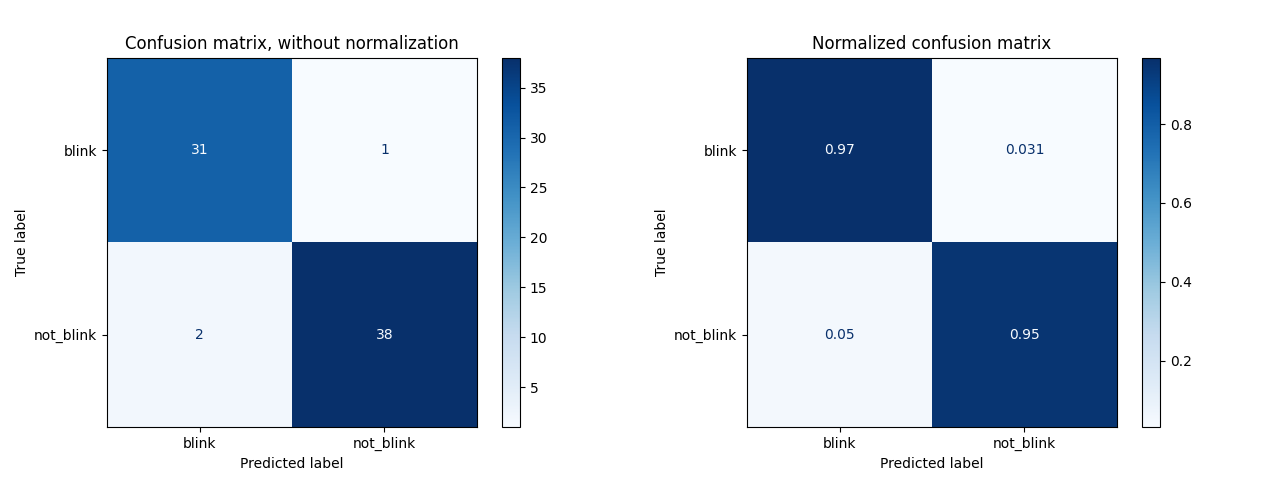
\includegraphics[width=\textwidth]{images/blink_confusion.png}
\caption{\textit{Confusion Matrix}-ok a \textit{Blink} adatkészletre}
\label{fig:blinkconfusion}
\end{figure}

A \textit{Blink} gesztus képe természetesen más módszerekkel is meghatározható, egy egyszerűbb megközelítése lehet a problémának a \textit{blob} alapű szűrés elvégzése. A \textit{blob} közös tulajdonság(okkal) rendelkező összefüggő pixelhalmaz. A közös tulajdonságok közé tartozhatnak a konvexitás, méret, alak, intenzitás-értékek, stb\ldots A \textit{Frame differencing} eljárás során keletkezett képen szabad szemmel is megfigyelhető, hogy az egyes \textit{Blink} gesztusok hol helyezkednek el, hiszen korábban megállapítottuk, hogy a kapott képen hasonló nyomot hagynak. Így a megfelelő paraméterekkel ellátott \textit{Blob detektor} segítségével meg lehetne határozni a \textit{Frame differencing} képén elhelyezkedő \textit{Blink} képeit. Ezen megoldás kétségkívül egyszerűbb megoldást jelentene, mint az általam használt eljárás, viszont a megfelelő paraméterek megválasztása időigényes feladat lehet. Az \textit{OpenCV}-ben található implementációt a \texttt{cv2.SimpleBlobDetector()} függvényben találhatjuk meg.

\SubSection{Drag and Drop}

A \textit{Drag} az elem elkapása utáni állapot jelenti, amikor a felhasználó az elkapott elem helyzetét szabadon változtathatja, majd új pozíciójára teheti (\textit{Drop}). Ennek a funkciónak a megvalósításához többféleképpen is hozzáláthatunk.

Az első ötletem szerint a vektormező vektorait felhasználva lokális eredővektor segítségével becsülte volna meg a program a mozgatandó virtuális elem új helyzetét. Ez a megoldás gyakorlatban az elvárásokat nem elégítette ki. Több probléma is adódott. A \textit{Rács} lyukacsossága miatt nem mindig esett vizsgálandó pont a mozgás helyére. Az egyes kiugró értékek is befolyásolták a végeredményt, a mozgatandó elemek ilyen esetekben gyorsabban mozogtak a vártnál. Ez a megoldás tehát nem tűnt stabilnak, a vektormező rácsának sűrítésével pedig a program jelentős lassulásba ütközött volna. Más megoldás után kellett kutatni.

Mivel a \textit{Drag and Drop}-ot előreláthatólag a prezentáló csak rövid időszakaszokban fogja használni, ezért a következő ötlettel áltam elő: a \textit{Blink} gesztus pozíciójára kontollpont(okat) illeszthetnénk, melyekre külön-külön elvégezhetnénk az \textit{Optical Flow} eljárást és a pont vagy a pontok súlypontjának pozíciója függvényében változna a mozgatandó virtuális elem pozíciója is. Már egyetlen kontrollpont használata is kielégítő eredményt adott. Több kontrollpont használata csupán csak a biztonság érdekében tűnik megfelelőnek. Ha esetleg egy pont új pozícióját rosszul becsülné meg az eljárás és a pont egy bizonyos ponton leragadna, akkor maradjanak olyan "tartalék" pontok is, amelyek biztosítanák a funkció helyes működését.

A követendő pont(ok) helyes megválasztásánál figyelembe vehetjük a \textit{Blink} képét. A képen megyfigyelhető legnagyobb intenzitásértékű pontok koordinátájának a súlypontját meghatározhatjuk, hogy az elhelyezendő pont a lehető legnagyobb valószínűséggel a prezentáló személy \textit{Blink} gesztust végrehajtó kézfejére essen. Viszont a \textit{Blink} gesztus kiszámolt középpontját is felhasználhatjuk erre a célra, hiszen már az is megfelelő pontosságot biztosít.

\SubSection{Rotation}

A \textit{Rotation} gesztus két tulajdonsággal íható le: ezen gesztusnak mindig létezik egy elméleti középpontja, ami körül történik az elmozdulás, valamint van iránya is.
Becslést adni a mozgás lehetséges középpontjának pozíciójára a vektormező elemzésével célszerű.
A vektorokhoz egyenes egyenleteket szerkeszthetünk. Az egyenes egyenletének egy pontja a vektor kezdőpontja lesz, a normálvektora pedig az egyenes irányvektora.

\begin{figure}[h]
\centering
\frame{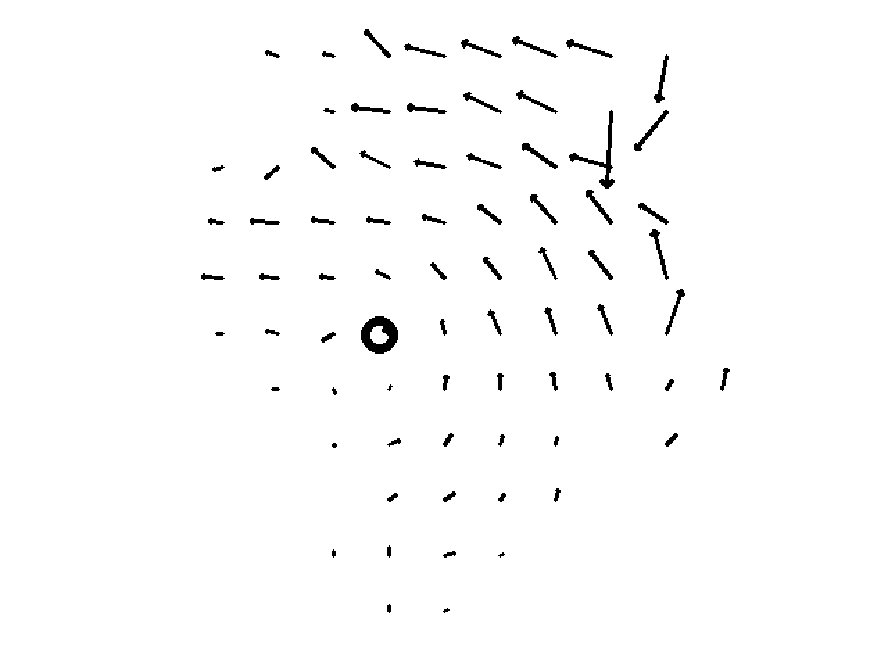
\includegraphics[width=8.88truecm, height=6.66truecm]{images/swirl_screenshot.png}}
\caption{A vektormező egy állapota a becsült forgási középponttal}
\label{fig:rotation}
\end{figure}

Két egyenletből álló egyenletrenszer megoldásaként megkapjuk az $x,y$ ismeretlen értékeket, melyek a két egyenes metszéspontjának a pozícióját adják meg.
A metszéspontokat számolva létrejön egy ponthalmaz, amelynek súlypontja az elméleti középpont közelében fog elhelyezkedni. A futásidő csökkentése érdekében érdemes csupán csak a szomszédos vektorok egyenleteit megoldani. A becslés pontossága viszont így romlani fog.
Ha pedig több \textit{Rotation} pontot is vizsgálni szeretnénk, akkor segítségül hívhatjuk a \textit{Hőtérkép}-ből kinyert vektorcsoportok halmazait, majd ezen csoportokon külön-külön elvégezhetjük az eljárást a lokális súlypontok után kutatva.

Az irány meghatározásához számolhatunk forgási szöget is. Ezt legegyszerűbben az \textit{arctg2} függgvénnyel tehetjük meg, amely segítségével a síkvektorok $y$ és $x$ koordinátáiból meghatározhatjuk az $x$-tengellyel bezárt szögüket.
\begin{align*}
		\text{arctg2$(y,x)$} =
  			\begin{cases}
    			\text{arctg$\left(\frac{y}{x}\right)$} & \text{, ha $x\geq \vert y \vert$,} \\
    			\frac{\pi}{2}-\text{arctg$\left(\frac{x}{y}\right)$} & \text{, ha $y\geq \vert x \vert$,}\\
    			-\frac{\pi}{2}-\text{arctg$\left(\frac{x}{y}\right)$} & \text{, ha $y\leq -\vert x \vert$,}\\
    			\pi+\text{arctg$\left(\frac{y}{x}\right)$} & \text{, ha $x \leq -y \leq 0$,}\\
    			-\pi+\text{arctg$\left(\frac{y}{x}\right)$} & \text{, ha $x \leq y \leq 0$}\\
  			\end{cases}
\end{align*}
% forrás? Wiki
A vizsgált vektorokra elvégézhetjük az \textit{arctg2}-t, majd átlagot vonva a kapott értékekből egy átlagos forgási szöget kapunk.

\SubSection{Többpontos kezelés}

A \textit{Hőtérkép}-et vizsgálva azonosíthatunk és elkülöníthetünk vektorok halmazait egymástól. Az így kapott csoportokat vizsgálva további funkciókat valósíthatunk meg. A több ponttal irányítható funkciók közé tartozhatnak a \textit{Widget}-eken végrehajtható különféle manipulációk, mint például a skálázás is. További komplexebb gesztusok felismeréséhez is felhasználhatnánk a pontok egymáshoz képesti vizsgálatából kapott eredményeket.
Minden vektorcsoporthoz tartozik egy-egy lokális eredővektorból számított irányvektor, mely a vektorcsoport elmozdulásának irányát mutatja.
A skálázás műveletéhez két vektorcsoportot feltételezve az alábbi módon vizsgálhatjuk a két pont egymáshoz képesti elmozdulását.
Irányok esetében $\vec{u},\vec{v}\in \mathbb{R^2}$ esetén
\begin{align*}
\vmatrix \vec{u}+\vec{v} \endvmatrix &< \varepsilon_{\text{irány}}\\
&\approx \vec{0}
\end{align*}
Amennyiben a két pont iránya teljesen ellentétes, akkor a kapott érték a null vektorhoz közelít. Érdemes normalizált vektorokat használni, ha csupán az elmozdulás irányát szeretnénk vizsgálni és az egyes lokális irányvektorok hosszától el szeretnénk tekinteni.

\SubSection{Symbol}

A prezentáló személy bizonyos mozdulatokat elvégezve további funkciókat érhet el. Az ilyen gesztusok egy fajtája általában a magyarázó mozgástól eltérőek, bizonyos pályákat követnek. Ilyen mozdulatok lehetnek például egy kör, vagy egy L betű, vagy különféle minták rajzolása levegőbe. Az egyes mozdulatok hasonló mintázatot követnek.

A dolgozat programjához mellékelt \textit{Symbol} adatkészlet három gesztus adatait tartalmazza. A három mozdulat a következő neveket kapta:
\begin{itemize}
	\item \textit{Gamma}
	\item \textit{Omikron}
	\item \textit{BRC} (Bottom Right Corner, vagyis jobb alsó sarok - az Unicode (U+231F) karakternek felel meg)
\end{itemize}
\begin{figure}[h]
\centering
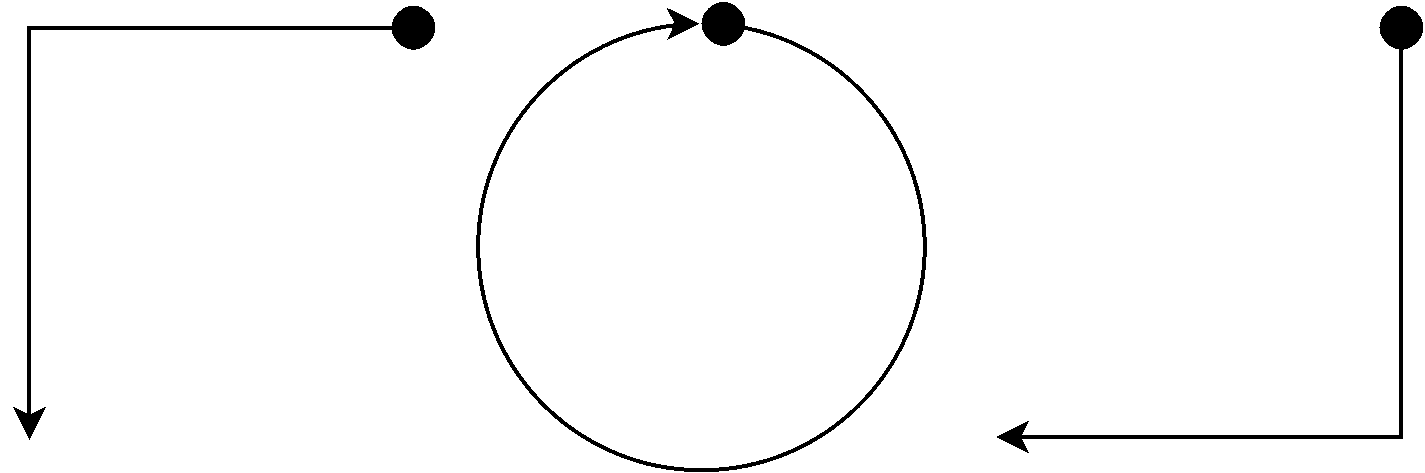
\includegraphics[width=10truecm]{images/symbols.png}
\caption{\textit{Gamma}, \textit{Omikron}, \textit{BRC}}
\label{fig:symbols}
\end{figure}

Ezen gesztusokra betanított osztályozó modell \textit{Confusion Matrix}-a a \ref{fig:confusionm} ábrán figyelhető meg. Belátható, hogy az osztályozó modell pontossága a minták között megfigyelhető viszonylag nagy távolságoknak is köszönhető.

Az ilyen típusú gesztusok felismeréséhez felhasználhatjuk az \textit{OCR}, vagyis az \textit{Optical Character recognition} (Optikai karakter felismerés) módszert is, mely írott karakterek felismerésére szolgál. 
Az OCR kipróbálásához rendelkezésre áll egy ingyenes adatkészlet is, a MNIST, amely 70.000 kisfelbontású képet tartalmaz írott számokról 0-9-ig. Segítségével különféle osztályozók taníthatók be, illetve az osztáyozók tejesítményének egyik mérőeszközévé vált az idők során. Az osztályozómodell betanításához a jellegvektorok értékeit a szürkeárnyalatos képek intenzitásértékei adják. Ha egy új osztályozó rendszert fejlesztenek, valószínűleg a MNIST adatkészlettel is kipróbálják azt. \cite{geron2019hands}

Mivel a probléma hasonlít az OCR-hez, hasonló megoldást alkalmazhatunk a levegőben leírt gesztusok felismeréséhez is. A mozdulat képét egy, a \textit{Hőtérképpel} megegyező méretű vászonra rögzíti a program. A vászon alapszíne fehér, vagyis 255 intenzitás értékekkel van ellátva. A gesztus képét a \textit{Hőtérkép} elemzésénel kinyert kontrollpontok rajzolják a vászonra: A vektorcsoportnak meghatározandó a súlypontja, mely a virtuális ecset hegyét jelenti. A súlypont elmozdulását a vásznon 0 intenzitásértékek követik, vagyis az elvégzett mozdulatok képei fekete színnel jelennek meg a vásznon. Mivel az egyes mozdulatok hasonló mintázatot követnek, a vásznon megjelenő képük is hasonló lesz.

\begin{figure}[h]
\centering
\frame{
\includegraphics[width=10truecm, height=7.33truecm]{images/OCR-Gesture.png}}
\caption{Egy levegőbe leírt \textit{Omikron} mintázata egy 11$\times$15-ös vásznon}
\label{fig:ocr-gesture}
\end{figure}

A vászon frissítése két módszerrel történik. Az elmozdulás értékek egy csúszóablakban helyezkednek el, amelyben maximum  30 érték kaphat helyet. Továbbá ha a \textit{Hőtérkép}-en nem figyelhető meg kontrollpont, az elmozdulás értékek törlése felgyorsul, míg a teljesen üres vásznot nem kapjuk.

A felismerés pillanatát feltételekhez kell kötnünk. A mozdulat rajzolatának végső formája akkor alakul ki, amikor a felhasználó befejezte az adott mozdulatot. Ilyen esetben a videófolyamon nem figyelhető meg további mozgás. Az időzítés egyik feltétele mindenképpen a mozgás hiányának kell lennie. Ez többféleképpen is megfigyelhető, vizsgálhatjuk a globális eredővektorunkat is, vagy a \textit{Hőtérkép} segítségével meghatározott csoportok számát is figyelembe vehetjük. Mivel a mintázat rajzolásához is a vektorok összetartozó csoportját használtuk fel, az időzítés egyik feltételének a vektorcsoportok hiányát szabhatjuk meg. Egy másik feltétel a rajzolat aktuális állapotára vonatkozhat. Figyelembe vehetjük a vonalhosszat is, vagyis egy bizonyos vonalhossz alatt nem végeznénk el az osztályozási becslést. Ezen két feltétel biztosítja, hogy az osztályozási művelet végrehajtása a megfelelő pillanatban történjen, elkerülve a felesleges számításokat, hibás becsléseket.

Mielőtt a gesztust reprezentáló képről döntene a modellünk, egy előfeldolgozási lépést kell végrehajtanunk rajta. A gesztus képe nem fogja betölteni a teljes vásznat, így sok felesleges értéket fog tartalmazni. Ennek kiküszöbölésére ki kell vágnunk a gesztus rajzolt képét és egy előre meghatározott felbontásra kell konvertálnunk. Tapasztalati alapokon a 11 $\times$ 15 -ös felbontás megfelelőnek tűnik, így minden egyes kivágott képet ilyen felbontásra kell alakítanunk. Ezen előfeldolgozási lépés elősegíti, hogy a betanított modellunket különböző rácsfelbontások és képarányok mellett is használni tudjuk, ugyanis a jellegvektorok mérete minden esetben azonos lesz.

\begin{figure}[h]
\centering
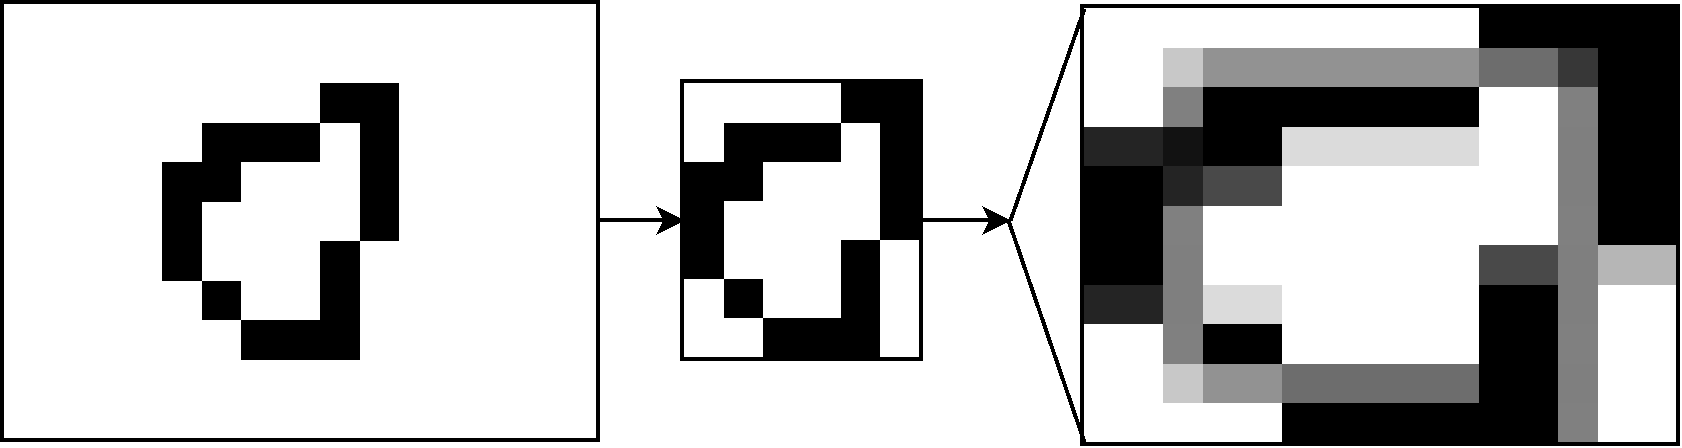
\includegraphics[width=10truecm]{images/crop_resize.png}
\caption{\textit{Symbol} előfeldolgozás}
\label{fig:symbol_pre}
\end{figure}

A mozdulat osztályozása utáni pillanatban a vásznat törölnünk kell, vagyis csupa 255 intenzitásértékkel kell ellátnunk, hogy a megszabott feltételek tovább ne teljesüljenek a további becsléseket elkerülve.

A modell betanításához képekre lesz szükségünk, amelyeket a programmal egyesével legyárthatunk és osztályozhatunk. További módszereket is használhatnánk a tanítóminta előállítására. Ilyenek lehetnek a minták generálása egy alap mintahalmazból zajosítással és egyéb megoldásokkal. Amint a minta rendelkezésünkre áll, a modell tanítható is.

A levegőben leírt gesztusok felismerése egy izgalmas kutatási terület, az általam elkészíett \textit{Optical Flow} megoldáson kívül is léteznek megközelítései. Általában a videófolyamon valamilyen szűrési technika segítségével kiemelik a megfigyelendő objektumot, valamilyen tulajdonsága alapján és a szűrt adatokon végzik el a további feldolgozási lépéseket. A szűrés történhet textúra, alak, mozgás, szín alapján is. \cite{fadhil2018trackingsurvey} Esetemben a mozgás alapján szerzett információk alapján történt a gesztus detektálása. A csupán mozgás alapú módszer hátrányai közé sorolhatjuk, bizonyos esetekben a pontatlanságot is, hiszen nincsen meghatározva pontosan a vizsgálandó objektum, így bármely megfigyelhető mozgásra képes aktiválódni. Viszont, más szemszögből nézve, ez a tulajdonság jelentheti a módszer előnyét is, hiszen így jobban alkalmazkodik a különböző bemenetekhez.

Kevert megoldásokkal is történhet a detektálás, például háttérmodell segítségével kivágott alak és a hozzátartozó elmozdulásértékek alapján rendkívül pontos gesztusfelismerő konstruálható. \cite{lin2009recognizing}

A gesztusfelismerést két csoportba sorolhatjuk: statikus és dinamikus. A statikus gesztusfelismerés alatt olyan megoldásokat értek, melyeknél nem játszik szerepet az idő. Vagyis például a detektálás a kézfej aktuális állása alapján történik. \cite{purohit2018precisehand} \cite{robust2017mouse} \cite{kumar2019calculator} Az ilyen típusú megközelítések nagy szerepet játszhatnak például a jelnyelv feldolgozásában is.

A dinamikus gesztusfelismerésnél az idő kulcs szerepet játszik. Az általam megalkotott módszer is ebbe a csoportba sorolható. Az ilyen megoldásokra jellemző, hogy a mozgást valamilyen módon rögzítik, különböző technikákkal lenyomatot készítenek a feldolgozás során kinyert adatok alapján és az így kapott mozgás képe alapján történik a detektálás. A mozgás rögzítése történhet a videó alapú megoldásokon kívül például gyroszkóppal ellátott speciális kesztyű segítségével is \cite{ponraj2012wireless}. Ha a videóalapú megoldásoknál maradunk, a csupán egy egyszerű kamera segítségével megvalósított megoldások viszonylag ritkák \cite{joseph2018visual}, az ilyen jellegű kutatásokhoz előszeretettel felhasználják a \textit{Kinect} kamerarendszert \cite{zhang2013new} \cite{tang2018structured}
Az dinamikus gesztusfelismerési módszerek jellemző alkalmazási területe a levegőbe írt karakterek/szimbólumok felismerése.

Természetesen mindegyik megoldásnak léteznek előnyei és egyben hátrányai is. Belátható, hogy univerzális megoldást találni a problémára nem lehet. Mérlegelni kell a rendelkezésünkre álló technikai lehetőségeinket és a felhasználási területből adódó igényeket is a használandó technika megválasztásánál.

\Chapter{Interaktív grafikus elemek}

\Section{Widget-ek}

A program használata során a felhasználó különféle virtuális interaktív grafikus elemekkel léphet kapcsolatba, segítségükkel irányíthatja a programot, befolyásolhatja a prezentáció menetét. Az elemek más-más funkcióval rendelkeznek. Megjelenítés szempontjából minden grafikus elem képek segítségével jelenik meg.

\begin{itemize}
	\item \textbf{Button}: Az egyik legegyszerűbb interaktív elem, egy virtuális nyomógomb, melyet megnyomva egy meghatározott funkciót érhetünk el.
	\item \textbf{Grabbable}: A prezentáló személy a \textit{Drag and Drop} gesztus-sorozat segítségével megtudja fogni az ilyen tulajdonsággal rendelkező elemeket, majd kívánt új pozíciójába helyezheti azt.
	\item \textbf{Shiftable}: A felhasználó \textit{Shift} gesztus segítségével léphet kapcsolataba az ilyen típusú elemekkel.
	\item \textbf{Openable}: Ezen elemek nyithatóak, zárhatóak.
	\item \textbf{Rollable}: Hosszú elem, amelynek csak egy része látszik és egy elképzelt ablakon keresztül láthatjuk a tartalmát. A felhasználónak lehetősége van megváltoztatnia a megjelenítendő képrészletet.
	\item \textbf{Scale}: Két képből áll össze, segítségével értékeket állíthatunk be.
	\item \textbf{Tuner}: Virtuális "potméter". A \textit{Rotation} gesztussal léphetünk kapcsolatba vele és értékeket állíthatunk be egy meghatározott tartományon.
\end{itemize} 

\SubSection{Button}

A \textit{Button} vagy \textit{Nyomógomb} működtetése rendkívül egyszerű. Aktiválásához a felhasználónak egyszerűen csak a gomb területére kell emelnie például a kézfejét, a gomb pedig egy bizonyos idő elteltével reagál.

A gombon belüli mozgás figyelésére segítségül hívhatjuk a \textit{Hőtérkép} csoportjait. Ha egy csoport súlypontja a gombon belül helyezkedik el, majd ha megszűnik (vagyis ha a csoporthoz tartozó valódi objektum abbahagyja a mozgását), akkor a megszűnt csoport súlypontjának a koordinátáira egy figyelendő pontot helyezünk. Ha a vizsgálandó pont kilép a gomb tartományából egy előre meghatározott időn belül, akkor nem történik semmi. Ha viszont a vizsgálandó pont a gomb területén belül marad, a gomb aktiválódik. 
Vagyis ez egy valós helyzetben a következőképpen nézhet ki: A felhasználó a gomb területére irányítja a kézfejét, a kézfejének apró mozdulatai (melyek nem figyelhetőek meg a \textit{Hőtérképen} a képzaj kiküszöbölése miatt) egy vizsgálandó pont segítségével lesznek követve, amely a már ismert \textit{Optical-Flow} technikával valósul meg.

A véletlen gombnyomás, nem kívánt viselkedés elkerülése érdekében időkeretet kell megszabnunk a vizsgálandó pont a gombon belül töltött idejére. Ezen időintervallumnak viszonylag rövidnek kell lennie, hogy a felhasználói élmény ne romoljon (ne kelljen várni túl sokáig a gombnyomásra), viszont nem lehet túl rövid ahhoz, hogy egy esetleges véletlen mozdulat aktiválni tudja. A helyes időkeret megválasztása a gomb méretétől is függhet. Tapasztalati adatok szerint 0.2-0.5 másodperc közötti időkeret használata megfelelőnek tűnik.

\SubSection{Grabbable}

A megfogható tulajdonsággal rendelkező objektumokat a felhasználó a képtartományon belül szabadon áthelyezheti kedve szerint. A művelethez egy \textit{Drag and Drop} gesztust-sorozatot kell végrehajtania. A \textit{Blink} gesztus kiadásakor minden esetben számolódik egy pozíció érték, amely a kézfej helyzetét kívánja megbecsülni. Ha ezen pont az elem területére esik, akkor a pontot innentől kezdve vizsgálandó pontnak kell tekintenünk. A pont helyzetének frissítése az \textit{Optical-Flow} technikával történik. Az elem új pozíciója a ponthoz képest módosul, vagyis az elem a felhasználó kézfejét követi.
Amint elnavigálta a kívánt pozícióba az új elemet a felhasználó, eg újabb \textit{Blink} gesztussal a helyére teheti azt.

Hogy az elem véletlenül se lépjen ki a videófolyamból, korlátoznunk kell a lehetséges mozgásterét a képtartományra. Vagyis az elem szélei nem mehetnek túl a kép szélein. Ezen megszorítás a többi elemre is vonatkozik.

\SubSection{Shiftable}

A tologatható elemekkel \textit{Shift} gesztus segítségével léphetünk kapcsolatba. Az irányukba történő mozgásra megeggyező irányú mozgással reagálnak. Működésére olyan hatás jellemző, mintha az elemet tologathatnánk.

\SubSection{Openable}

Ezen virtuális elemek megjelenés szempontjából hasonlítanak egy pargamen tekercshez, belső tartalmuk kezdetben rejtett, azonban a felhasználónak lehetősége van kinyitni, megmutatva a belső tartalmát, majd becsukni az adott elemet.

A \textit{Tologatható elemekhez} hasonlóan, \textit{Shift} gesztussal léphetünk kapcsolatba az ilyen tulajdonságokkal ellátott elemekkel, viszont az ilyen típusú elemek mozgása egy bizonyos tengelyre korlátozódik, kezdőpozícióját megtartja és a megjelenítendő képrészlet nagysága változik csupán. Az elemhez definiálnunk kell a \textit{header} szekció méretét, ami az elem minimum méretét fogja megadni. Mivel az elem viselkedését a vektormező adataiból számoljuk, ezért a \textit{header} mérete nem lehet kisebb a rács sűrűségéből számított lépésköznél, hiszen ilyenkor bizonyos esetekben az elem becsukott állapotban egyetlen kontrollpontot sem fedne le, így a felhasználó nem tudna interakcióba lépni vele.
Az elem tényleges mérete pedig a teljesen kinyitott állapototára vonatkozik.

\SubSection{Rollable}

Néhány gondolat a \textit{Tekerhető elemekről}.

\SubSection{Scale}

Néhány gondolat a \textit{Csúszkákról}.

\SubSection{Tuner}

A \textit{Tuner} widget-et működése és megjelenése szempontjából egy potméter gombnak képzelhetjük el. Segítségével a felhasználó különböző értékeket állíthat be.
Az ilyen típisú widgeteket a \textit{Rotation} gesztus segítségével érhetjük el. Ha a \textit{Rotation} becsült forgási középpontja az adott elem belsejébe esik, az aktiválódik és a gesztus feldolgozása során további információkat figyelembe véve változik meg az állapota.

A felhasználó definiálhatja, hogy az egyes ilyen típusú widget-ek értékei milyen tartományon szerepelhetnek, vagyis meg kell határoznia a legkisebb és legnagyobb értéket, amelyet a widget felvehet. Az értékek számítása a forgási szög függvényében történik. A widget élete során kapott elfordulás szögei szummázódnak és a widget értéke ezen szummázott szög alapján számolódik. A szummázott összegre vonatkozik egy olyan megszorítás, hogy értéke, fokokban nézve, nem lehet 0$^{\circ}$ alatt és 360$^{\circ}$ fölött. Egy tomptó értéket is be kell vezetnünk, amellyel a szummázás előtt az eredeti szög értékét csökkentjük. Ez az érték tapasztalata alapokon 10, vagyis a tényleges becsült forgási szög tizedét vesszük csak figyelembe a finomabb működés érdekében.
Megjelenés szempontjából a \textit{Tuner} widget valóban elfordul. A hatás eléréséhez minden iterációban a widget súlypontját és a szummázott szöget felhasználva affin transzormációval elforgatjuk a widget eredeti képét.

\Chapter{Megvalósítás}

\Section{Az \texttt{arpt} csomag felépítése}

% TODO: Osztályok felsorolása.

\Section{Videóeszköz kezelése}

Capture device-al kapcsolatos dolgok

\Chapter{Prezentáció példák}

% TODO: Tutorial jelleggel leírni, és bemutatni, hogy hogy lehet használni az alkalmazást.

A program jelenlegi verziójához nincs mellékelve grafikus felülettel ellátott projekt-szerkesztő, viszont a projekt sturktúra szabályait követve létrehozhatunk új prezentáció leíró állományokat.

\bigskip

\dirtree{%
.1 /presentation\_project01.
.2 /images.
.3 button.png.
.3 tuner.png.
.3 \ldots.
.2 /preferences.
.3 canvasses.json.
.3 settings.json.
.3 windows.json.
.2 scene.json.
.2 actions.py.
}

\bigskip

\noindent A projekt fájl \textit{JSON} állományokból, képekből és egy \texttt{actions.py} modulból áll, amelyben leírásokat adhatunk a \textit{Button} és a \textit{Tuner} widgetek viselkedésére.

A \texttt{/preferences} jegyzékben pedig általános beállításokra vonatkozó leírásokat adhatunk meg. A \texttt{settings.json}-ben a \textit{videófolyam}, a \textit{Rács} és a \textit{Hőtérkép} paramétereit adhatjuk meg. A
\texttt{canvasses.json}-ben pedig, ha igényt tartunk rá, a \textit{Vektormező} és a \textit{Globális eredővektor grafikon} vásznak tulajdoságait állíthatjuk be.
A \texttt{windows.json}-ben pedig az OpenCV által megjelenítendő ablakokat állíthatjuk be. A prezentációs során csak egy teljesképernyős ablakra van szükségünk, melyben a kimeneti képet láthatjuk. Ha csak az eredmény érdekel bennünket és nem tartunk igényt a program működésének megfigyelésére, akkor az utóbbi két fájl akár üresen is hagyható.

A \textit{DataParser} egység feldolgozza a felhasználó projekt fájlait és a bennük található leírások szerint futtatja a programot.

A \texttt{scene.json} állományban definiálhatjuk az egyes diák tartalmát. Az állomány egy lista, melynek elemei a \textit{JSON} objektummal leírt diák. A jelenlegi verzióban csupán egyetlen mezőt tartalmaznak a diákat leíró objektumok, a \texttt{widgets}-et. Ha később további információkkal szeretnénk ellátni a diákat (például metadatokat, egyéb leírásokat, további funkciókat szeretnénk jelölni), ezen a szinten tehetjük meg. A \texttt{widgets}-en belül pedig a widgetek listáját találjuk. Az egyes widget típusok különféle paraméterekkel rendelkeznek.\\
Példaként tekintsünk egy egyetlen diával rendelkező \texttt{scene.json} állományt, melyen egyetlen \textit{Tuner} widget helyezkedik el:
\begin{verbatim}
[
    {
        "widgets": [
            {
                "type":        "Tuner",
                "position":    [420, 300],
                "dimension":   [150, 150],
                "image":       "images/tuner.png",
                "min_value":   80,
                "max_value":   200,
                "transparent": true,
                "action":      "sample_action$arg"
            }
        ]
    }
]
\end{verbatim}
Jól látható, hogy a widgeteket \textit{JSON} objektumokként írhatjuk le, \texttt{type} mezőben jelöljük a widget típusát, az utána következő mezőkben pedig a widget paramétereinek értékeit adhatjuk meg. A \texttt{transparent} mezőben jelölhetjük, hogy kívánjuk-e használni a widget képének $\alpha$ csatornáját. Ha \texttt{true} értékkel látjuk el ezt a mezőt, akkor a program $\alpha$ csatornával eggyütt olvasssa be a képet, \texttt{false} esetén pedig csupán csak a három színcsatornára számít. Az $\alpha$ csatornával ellátott widget képek az $\alpha$ értékeiknek megfelelően rajzolódnak ki.
Az \texttt{action} mezőben pedig a widget-hez tartozó függvény nevét jelölhetjük, az \texttt{actions.py}-ból, illetve a \texttt{\$} szimbólum után egy további adatot is megadhatunk argumentumként, melyet stringként olvas be a \textit{Parser}. Ezt az adatot a futás során bármilyen formában felhasználhatjuk a widgethez tartozó függvényen belül.

A következőkben két példa prezentáción keresztül szeretném bemutatni a program lehetséges használati módjait. Az első példa prezentációban pár képfeldolgozó módszer kerül bemutatásra, a második pedig a dolgozatomról szól.
A videófolyamon megjelenő widget-ek képeit \textit{GIMP (GNU Image Manipulation Program)} képszerkesztő segítségével szerkesztettem meg. Az elkészült képek csupán szemléltetésre szolgálnak. Minőségi, szemetgyönyörködtető, alfa csatornával rendelkező widgetek használatával még látványosabbá tehetjük a prezentációnkat. Egy egységesített, felhasználóbarát widget szerkesztő megoldhatná a külső képszerkesztő használata során adódó kényelmetlenségeket. A szöveg helyét néhány helyen a \textit{Lorem ipsum} szövegrészlet vagy angol nyelvű szöveg tölti ki.

\Section{Képfeldolgozás, OpenCV bemutatása}

Az első példaprezentáció a képfeldolgozás témakör köré épül és bemutatásra kerül az \textit{OpenCV} is. A programom segítségével a témakört egy új megközelítésben ismertethetjük. Az egyes képfeldolgozó technikákat valós időben mutathatjuk be, a videófolyamot manipulálva, dinamikus paraméterezés mellett. Az így megvalósított prezentáció, látványosabb és kifejezőbb, szemléletesebb lehet a hagymányos prezentációs eszközökkel megvalósított előadásoknál.

Összeállításánal igyekeztem kihasználni a programom edddig elkészült állapotainak lehetőségeit. A widgetek paramétereit a fejezet bevezetésében leírtak alapján állítottam be a \texttt{scene.json} állományban. Az állomány tíz darab objektuma a tíz fóliát jelöli.\\
A diasor szerkezete a következő:
\begin{itemize}
	\item Bevezetés
	\item Menü
		\begin{itemize}
			\item Digitális képek
			\item \textit{Alpha Blending}
			\item Küszöbölés technika
			\item Éldetektálás
			\item Különböző filterek/szűrők bemutatása
				\begin{itemize}
					\item Gauss-elmosás
					\item Hisztogram kiegyenlítés
				\end{itemize}
		\end{itemize}
	\item Befejezés
\end{itemize}
Mint láthatjuk, a prezentációnak különböző szintjei vannak. A prezentációról egy képernyőképet \aref{fig:opencvdemo}. ábrán láthatjuk.

\begin{figure}[h]
\centering
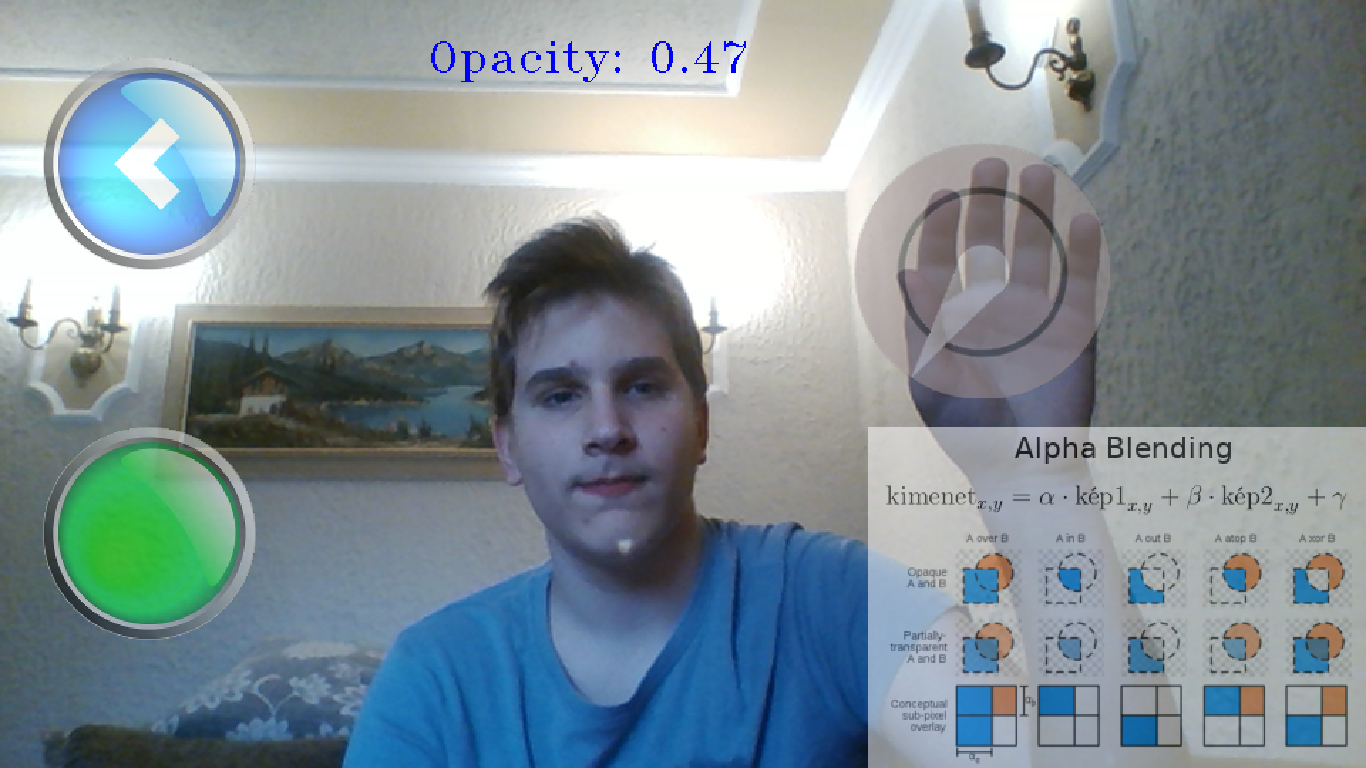
\includegraphics[width=\textwidth]{images/opencv_demo_screenshot.png}
\caption{Képernyőkép a demoról}
\label{fig:opencvdemo}
\end{figure}

Az első dián szereplő \textit{Rollable} widget tartalmazza a bevezetést, amely egy rövid áttekintés, hogy miről is fog szólni a prezentáció. Egy \textit{Shiftable} típusú \textit{OpenCV} logó is helyet kapott itt, illetve egy \textit{Button} típusú widget, melynek a funkciója a léptetés, melynek függvénye az \texttt{actions.py} modulon belül található meg. A prezentációban szereplő léptetést a \texttt{scene.json} állományban a következő módon jelölhetjük:
\begin{verbatim}
"action": "jump_to$1"
\end{verbatim}
Bárhol járjunk az előadásban, a fenti jelöléssel ellátott \textit{Button} az 1-es indexű fóliára fog eljuttatni minket. A \texttt{jump\_to} függvény pedig a következőképpen néz ki:
\begin{python}
def jump_to(controller, button_widget):
    if button_widget.pushed:
        controller.current_scene = int(button_widget.arg)
        button_widget.pushed = False
\end{python}
A függvény paramétereként átadódik a \texttt{controller} és a \texttt{button\_widget} címe, melyeket elérve módosíthatjuk a program aktuális állapotait. Ha ezen funkcióval ellátott \textit{Button} típusú gomb lenyomódik, akkor az éppen aktuális fólia sorszámát manipuláljuk az argumentumként kapott adattal, melyet \texttt{int} típusúvá, azaz egész számmá konvertálunk. A művelet végén a gomb lenyomását megszűntethetjük, így ha vissza kell lépnünk erre a fólira, nem okoz majd gondot a lenyomva maradt gomb, amely a fóliára lépés pillanatában újra elnavigálna a benne jelzet fóliára.
A példaprezentációra jellemző, hogy előre és hátra is léptethetjük a fóliákat, így bejárva az összes szintet.

A második fóliát egy menürendszernek szántam. A csempeszerűen elhelyezkedő widgetek segítségével érhetjuk el rajtuk jelölt funkciókat. A diavetítés így nem lineáris lesz, hiszen szabad sorrendben lefuttathatjuk azokat. Ezen widgetek \textit{Button} típusúak, a hozzájuk tartozó művelet pedig az aktuális diát jelző pointer értékének változtatása a cél helyre, vagyis a már említett \texttt{jump\_to} függvénnyel való ugrás. Ezen diák szintén a \texttt{scene.json} elemei, sorban, a Menü fólia után helyezkednek el.

Az Menüből elérhető diák tartalma változó, a hozzájuk tartozó témakör kifejtését tartalmazzák. A dinamikus elemekkel ellátott diákon a témakörnek megfelelően elhelyzetem olyan vezérlőket, melyekkel manipulálhatjuk a kimeneti videófolyamot a témakörök szemléletesebb bemutatása érdekében.
Például a Küszöbölés technikát bemutató dián a funkciót aktiváló \textit{Button} megnyomása esetén a videófolyamon a \textit{Tuner} értékeinek megfelelően végrehajtódik a küszöbölés művelete. A \textit{Tuner} segítségével állíthatjuk a küszöb alsó határát, az eljárás szemléltetése érdekében.
Az éldetektálással és \textit{Alpha Blending} technikákkal foglalkozó fóliákon szintén hasonlóan demonstrálhatjuk a technikák működését, \textit{Tuner} widget segítségével értékeket állítva.
A filtereket bemutató fólia szintén egy menürendszer, melyen két \textit{Button} segítségével érhetejük el a kívánt fóliákat. A Gauss-elmosást és a hisztogram kiegyenlítést bemutató fóliákon található egy-egy \textit{Button} widget is, melynek megnyomása esetén a hozzátartozó művelet végrehajtódik. Például a Gauss-elmosással foglalkozó fólia ilyen \textit{Button}-ja a következő egyszerű függvénnyel rendelkezhet:
\begin{python}
def gauss_button(controller, button_widget):
    if button_widget.pushed:
        controller._video.frame = \
        		cv2.GaussianBlur(controller._video.frame,
					(19, 19),
					cv2.BORDER_DEFAULT)
\end{python}
A videófolyam aktuális képkockáját felülírjuk a \texttt{cv2.GaussianBlur()} kimenetével. Mivel a projektben definiált függvények lekezelése a feldolgozási folyamatok után történnek meg, így az ilyen módon módosított képkocka ezután csupán már csak megjelenítésre vár.

A módszereket bemutató diák mindegyikén elhelyezkedik egy-egy \textit{Button} típusú widget is, amellyel az eggyel korábbi szintre, vagy a Menübe léphetünk vissza.

A Menüből pedig szintén egy \textit{Button} segítségével léphetünk tovább az utolsó diára, ahol egy \textit{Expandable} widget segítségével foglalhatjuk össze a prezentációnkat és köszönhetjük meg a figyelmet.

\Section{Dolgozat bemutatása}

A második példaprezentáció segítségével a dolgozatomat szeretném bemutatni.
A prezentáció során a videófolyam az általános widgetek mellett valós időben frissülő ábrákkal is kiegészül, melyeket egyébként a program fejlesztői módú futása során láthatnánk. Ilyenek a \textit{Frame Difference}, \textit{Grab}, \textit{Vektormező} ábrák. A folyton frissülő ábrák segítségével a dolgozat kulcs elemeit szemléletesebben bemutathatjuk.

A prezentációban a dolgozatomban tárgyalt főbb elemek kerülnek említésre. A fejezetek szerint haladva kerül bemutatásra a témakör és a dolgozat anyaga. Egyedül a widgetek nincsenek külön bemutatva, hiszen azok a prezentáció teljes egészében jelen vannak. Az egyes fóliák közti léptetés az előző prezentációhoz hasonlóan van megoldva. A widgetek \textit{design}-ja is hasonló, viszont ennél a prezentációnál mellőztem a \textit{Lorem ipsum} és angol nyelvű szövegeket a tartalomelemeknél és törekedtem az informatív leírásokkal és szemléletes képekkel színesíteni a widgeteket.

Az első példaprezentációban használt menürendszeres megoldást itt is szeretném alkalmazni a prezentációk megszokott linearitását megtörve. Természetesen a prezentáció ajánlott menete így is lineáris marad, ez a fajta öszzeállítása az előadásnak csupán azért szükséges, hogy a logikailag egybefüggő részek még jobban elkülönüljenek egymástól. A fő fóliákból további alfóliák érhetők el. Nem célom labirintusszerűen felépíteni az előadást, hogy a prezentáló személy se tudjon kiigazodni a saját előadásában, így a lehetséges mélységi szintet minimalizálni fogom.\\
A prezentáció szerkezete a következő:
\begin{itemize}
	\item Bevezetés
	\item Koncepció
		\begin{itemize}
			\item Kiterjesztett valóság
			\item Prezentációs szoftverek
			\item \textit{OpenCV} és \textit{scikit-learn}
		\end{itemize}
	\item Gesztusok
		\begin{itemize}
			\item Optical-Flow
			\item \textit{Grid}/vektormező
				\begin{itemize}
					\item \textit{Sweep}
					\item \textit{Rotation}
					\item \textit{Shift}
				\end{itemize}
			\item \textit{Hőtérkép}
				\begin{itemize}
					\item \textit{Blink}
					\item \textit{Symbol}
				\end{itemize}
			\item Gépi tanulás
		\end{itemize}
	\item Példa prezentációk
	\item Összegzés, befejezés
\end{itemize}
Mint látható, különböző szinteket különíthetünk el. Az egyes szintek gyökéreleméhez egyetlen lépéssel vissza tudunk lépni, viszont a fóliákból a velük egy szinten lévő további fóliákat nem érjük el közvetlenül. Kivételt képeznek ez alól a legfelső szinten elhelyezkedő diasorok, közöttük szabadon lépkedhetünk.

A Bevezetés fóliában egy általános bevezetés megtételére van lehetőségünk. Említésre kerülhet a dolgozat feladata, melyet a későbbiekben részletesebben is ismertethetünk. Hasonlóan az első prezentációhoz, itt is egy \textit{Rollable} widgeten helyezkedik el a bevezetés tartalma.

\begin{figure}[h]
\centering

\includegraphics[width=\textwidth]{images/dolgozat_demo_screenshot.png}
\caption{Képernyőkép a demoról}
\label{fig:dolgozatdemo}
\end{figure}

A bal alsó sarokban elhelyezkedő \textit{Button} segítségével érhetjük el a következő diát, a Koncepció menüjét (\ref{fig:dolgozatdemo}. ábra), amelyről további fóliákat érhetünk el. Itt taláható meg a kiterjesztett valóság, prezentációs szoftverek, \textit{OpenCV} és \textit{scikit-learn}-el foglalkozó diasorok. Az itt szereplő widgetek még nem tartalmaznak élő-ábrákat, az általános widgetek segítségével mutthatjuk be az adott témaköröket. Ezen szekció célja az említett fogalmak tisztázása, általános bemutatása.

A Gesztusok fólia szintén egy menürendszert tartalmaz. Innen 4 további fóliát érhetünk el.
Itt találjuk meg az \textit{Optical-Flow}, a \textit{Grid}, a \textit{Hőtérkép} és a \textit{Gépi tanulás} diasorokat. A \textit{Grid} és \textit{Hőtérkép} fóliákkal egy újabb szintet érhetünk el. A hozzájuk kapcsolódó témaköröket belőlük tudjuk elérni. Itt már megjelennek a frissülő ábrák is, melyek segítségével szemléltesebben be tudjuk mutatni az adott témát.
A \texttt{scene.json} állományban a gomb argumentumaként megadott "default" kulcsszó segítségével a gombokon belüli funkció gombnyomás nélkül is elérhető lesz. Ezen apró trükk segítségével a diára lépés pillanatában megjelennek az élő ábrák. A "default" kulcs megléte az \texttt{actions.py} modulon belül található függvényekben kerül ellenőrzésre. Ez csupán csak egy példa az argumentum használatra. Amennyiben elmarad a kulcsszó a leíró állományban, a widget a gombnyomás után kezdi el frissíteni a saját képét a kívánt ábrára.

A példaprezentációkat tartalmazó fólia csupán csak említés szinten foglalkozik a példákkal. Az első példa widgetje \textit{Widget} típusú, vagyis semmilyen tulajdonsággal nem rendelkezik, csupán egy képet tudunk megjeleníteni a segítségével. A Dolgozattal foglalkozó példaprezentáció widget-je pedig egy \textit{Button}, melyet megnyomva visszatérhetünk a prezentáció legelső diájára.

A második példaprezentáció is hasonlóan ér véget, mint az első, egy \textit{Expandable} widget segítségével foglalhajuk össze az előadást és köszönhetjük meg a figyelmet.

\Chapter{Összefoglalás}

Hasonló szerepe van, mint a bevezetésnek.
Itt már múltidőben lehet beszélni.
A szerző saját meglátása szerint kell összegezni és értékelni a dolgozat fontosabb eredményeit.
Meg lehet benne említeni, hogy mi az ami jobban, mi az ami kevésbé jobban sikerült a tervezettnél.
El lehet benne mondani, hogy milyen további tervek, fejlesztési lehetőségek vannak még a témával kapcsolatban.


\clearpage

\addcontentsline{toc}{chapter}{Irodalomjegyzék}
\bibliographystyle{plain}
\bibliography{dolgozat.bib}

\newpage

\pagestyle{empty}

\noindent \textbf{\Large A melléklet tartalma}

\vskip 1cm

\noindent A dolgozathoz tartozó melléklet az alábbi elemeket tartalmazza.
\begin{itemize}
\item A dolgozatot PDF formában.
\item A dolgozat \LaTeX\ forráskódját a \texttt{szakdolgozat} jegyzékben.
\item Az elkészített programot, benne az \texttt{arpt} könyvtárral a \texttt{program} nevű jegyzékben.
\end{itemize}

\bigskip

\noindent A dolgozat és az elkészített programok forráskódja \texttt{GitHub}-on, az alábbi címen elérhető:

\bigskip

\quad \url{https://github.com/DanielNagy97/szakdolgozat}

\pagebreak

\emph{A cikkben/előadásban/tanulmányban ismertetett kutató munka az
EFOP-3.6.1-16-2016-00011 jelű „Fiatalodó és Megújuló Egyetem –
Innovatív Tudásváros – a Miskolci Egyetem intelligens szakosodást
szolgáló intézményi fejlesztése” projekt részeként – a
Széchenyi 2020 keretében – az Európai Unió támogatásával, az
Európai Szociális Alap társfinanszírozásával valósul meg"}


\end{document}
